
\documentclass[a4paper,11pt]{article}
% Document line spacing
\usepackage{setspace}
% Maths resource packages
\usepackage{amsmath,amssymb,amsfonts,amsthm}
% Packages to allow inclusion of graphics
\usepackage{graphicx}
% Literature reference style
\usepackage[authoryear]{natbib}
\usepackage[bf]{caption}
% Display URLs correctly
\usepackage{url}
% Code display
\usepackage[outputdir=build]{minted}
\usepackage{xcolor}
% Import csv-files for tables
\usepackage{csvsimple}
% Round numbers (in tables)
\usepackage{siunitx}
% Display sideways figures (landscape mode)
\usepackage{rotating}
% Enforce line breaks
\usepackage[breakall]{truncate}
% Align decimal points in tables
\usepackage{dcolumn}
\newcolumntype{.}{D{.}{.}{-1}}
% Align footnotes (no indent of first line)
\usepackage[bottom,flushmargin,hang,multiple]{footmisc}
% Write pseudo code
\usepackage{algorithm}
\usepackage{algpseudocode}
\usepackage{etoolbox}
\usepackage{tabularx}
% Create tables with cells over multiple rows and columns
\usepackage{multirow, multicol}
% Include appendix sections in the TOC
\usepackage[toc]{appendix}
% Control behaviour of floating graphics, tables etc.
\usepackage{float}
% Create hyperlinks in cross references (for tables etc.)
\usepackage{hyperref}
% Correctly print "tilde" character
\usepackage{textcomp}
\newcommand{\textapprox}{\raisebox{0.5ex}{\texttildelow}}
% Widow and orphan control (single lines at start or bottom of page)
\usepackage[all]{nowidow}

% -----------------------------
% --- user-defined commands ---
% -----------------------------

% insert Quantnet logo
\newcommand{\quantnet}{\raisebox{-1pt}{\includegraphics[scale=0.05]{thesis/figures/qletlogo.pdf}}\,}

% display vectors as bold symbols without arrow as superscript
\renewcommand{\vec}[1]{\boldsymbol{#1}}

% add possessive 's to author name in citation
\newcommand\cites[1]{\citeauthor{#1}'s\ (\citeyear{#1})}

% define arg min with underscored argument
\DeclareMathOperator*{\argmin}{\arg\min}

% enable "short" URLs without https:// or www part
\newcommand\rurl[1]{%
  \href{https://#1}{\nolinkurl{#1}}%
}

% Hyphenation of new words
\hyphenation{block-chain}

% --------------------------
% --- layout definitions ---
% --------------------------

% define topline
\usepackage[automark]{scrpage2}
\pagestyle{scrheadings}
\automark{section}
\clearscrheadings
\ohead{\headmark}

% define bibliography style
\bibliographystyle{agsm_edited}
\renewcommand{\harvardurl}[1]{URL: \url{#1}}
\renewcommand*{\UrlFont}{\itshape}

% define page size, margin size
\setlength{\headheight}{1.1\baselineskip}
\voffset=-3cm
\hoffset=-3cm
\textheight24cm
\textwidth16cm
\topmargin1cm
\oddsidemargin3cm
\evensidemargin3cm

% define line spacing = 1.5
\spacing{1.5}

% set line spacing for algorithms
\makeatletter
\expandafter\patchcmd\csname\string\algorithmic\endcsname{\itemsep\z@}{\itemsep=1.5ex}{}{}
\makeatother

% set indent manually in algorithm environment
\makeatletter
\newcommand{\multiline}[1]{%
  \begin{tabularx}{\dimexpr\linewidth-\ALG@thistlm}[t]{@{}X@{}}
    #1
  \end{tabularx}
}
\makeatother

% define space between text and footnote line
\addtolength{\skip\footins}{2pc plus 5pt}

% define space between footnotes
\setlength{\footnotesep}{1em}

% define second level for 'itemizing'
\renewcommand{\labelitemii}{-}

% Minted configuration
\definecolor{friendlybg}{HTML}{f0f0f0}

\setminted[r]{style=friendly, bgcolor=friendlybg,
breaklines, linenos}

\setminted[java]{style=friendly, bgcolor=friendlybg,
breaklines, linenos}



% ----------------------------------
% --- additional global settings ---
% ----------------------------------

% Number equations by sections
\numberwithin{equation}{section}

% Number figures by sections
\numberwithin{figure}{section}

% Number tables by sections
\numberwithin{table}{section}



% --------------------------------------
% --------------------------------------
% --------------------------------------
% --- the structure this tex document ---
% frontmatter:
%   - titlepage,
%   - acknowledgement,
%   - abstract,
%   - table of contents,
%   - list of abbreviations,
%   - list of figures,
%   - list of tables.
%
% body of the thesis:
%   - introduction,
%   - methods,
%   - data,
%   - results,
%   - conclusion,
%   - literature,
%   - appendix (figures, tables).
%
% last page:
%   - declaration of authorship.
% --------------------------------------
% --------------------------------------
% --------------------------------------




\begin{document}

% -------------------------------
% --- frontmatter: Title page ---
% -------------------------------

\thispagestyle{empty}
\begin{center}
\vspace{1cm}

    {\Large{\bf Forecasting in blockchain-based smart grids: Solving a prerequisite for the implementation of local energy markets}} \vspace{1cm}


    {\normalsize Master's Thesis submitted\\\vspace{0.5cm}
    to}\\\vspace{0.5cm}
    {\normalsize{\bf Prof. Dr. Wolfgang H\"ardle}} \\\vspace{0.5cm}
    {\normalsize Humboldt-Universit\"at zu Berlin \\
    School of Business and Economics \\
    Ladislaus von Bortkiewicz Chair of Statistics} \vspace{1cm}
    
    \includegraphics[]{thesis/figures/logo.pdf}
    \vspace{1cm}

    {\normalsize by \\\vspace{0.5cm}
    {\bf Michael Kostmann} \\
    (550961)} \vspace{1cm}


    {\normalsize in partial fulfillment of the requirements \\
    for the degree of \\
    {\bf Master of Science} \\
    in Economics and Management Science \\\vspace{1cm}
    Berlin, November 12,  2018}

\end{center}




% -----------------------------
% --- frontmatter: Abstract ---
% -----------------------------
\newpage
\pagestyle{plain}
\pagenumbering{roman}   % define page number in roman style
\setcounter{page}{1}    % start page numbering
\section*{Abstract}

Local energy markets (LEM) have been proposed as a solution to the challenges introduced by the current transformation of the energy landscape towards more distributed and volatile energy production from renewable energy sources. Blockchain-based LEM take the proposed solution one step further and implement the market mechanism as a smart contract. This makes a central authority coordinating the LEM obsolete. The proposed blockchain-based LEM rely on accurate forecasts of individual households' energy consumption and production to trade in the LEM. In a majority of the literature, such accurate forecasts are simply assumed to be given. The present research tests this assumption by evaluating the forecast accuracy achievable with current state-of-the-art energy forecasting techniques for individual households. In a second step the effect of prediction errors made by the best performing forecasting technique on market outcomes is assessed in three different supply scenarios. The evaluation shows, that although a LASSO regression model is capable of achieving reasonably low forecasting errors, the costly settlement of prediction errors can offset and even surpass the savings brought to consumers by a blockchain-based LEM. This shows that prediction errors can make the participation in LEM uneconomical for consumers, and thus, has to be taken into consideration in future research on blockchain-based LEM.

%%%%%%%%%%%%%%%%%%%%%%%%%%%%%%%%%%%%%%%%%%%%%%%%%%%%%%%%%%%%%%%%%



% -----------------------------
% --- frontmatter: Contents ---
% -----------------------------
\newpage
\tableofcontents
\clearpage


% ------------------------------------
% --- frontmatter: List of Figures ---
% ------------------------------------
\newpage
\addcontentsline{toc}{section}{List of Abbreviations}
\ohead[]{LIST OF ABBREVIATIONS}
\section*{List of Abbreviations}

%\begin{multicols}{2}
\begin{tabular}{rp{0.2cm}lp{1cm}rp{0.2cm}l}
    LEM     & &  Local energy market           \\
    RNN     & &  Recurrent neural network      \\
    LSTM    & &  Long short-term memory        \\
    LASSO   & &  Least absolute shrinkage and selection operator
\end{tabular}
%\end{multicols}



% ------------------------------------
% --- frontmatter: List of Figures ---
% ------------------------------------
\newpage
\addcontentsline{toc}{section}{List of Figures}
\ohead[]{\rightmark}
\listoffigures



% -----------------------------------
% --- frontmatter: List of Tables ---
% -----------------------------------
\newpage
\addcontentsline{toc}{section}{List of Tables}
\listoftables



% -------------------------------
% --- main body of the thesis ---
% -------------------------------
\newpage
\pagestyle{plain}
\setcounter{page}{1}    % start page numbering anew
\pagenumbering{arabic}  % page numbers in arabic style

\section{Introduction}\label{Sec:Intro}



%%%%%%%%%%%%%%%%%%%%%%
%%%   Motivation   %%%
%%%%%%%%%%%%%%%%%%%%%%

\subsection{Motivation}\label{Sec:Intro;Subsec:Motivation}

The increasingly wide-spread installation of renewable energy generators currently transforms the German energy landscape substantially \citep{Bayer:2018}. Already in 2017, more than 1.6 million photovoltaic micro-generation units were installed in Germany, according to the Bundesverband Solarwirtschaft \citeyearpar{BSW-Solar:2018}. This increasing amount of distributed renewable energy resources combined with a more volatile energy consumption of households –-- e.g., due to uncontrolled electric vehicle charging that can increase peak consumption \citep{Fitzgerald:2016,Floch:2017} --– presents a serious challenge for grid operators. As energy production and consumption have to be balanced at all times in any electricity grid \citep{Weron:2006}, the increasingly volatile and hard to predict energy consumption and production in low voltage grids requires new technological solutions to manage grid load and energy distribution.

Fortunately, the technological advancement that lead to the increasing complexity in the energy landscape, also opens up new opportunities to increase the efficiency and reliability of distributed renewable energy production and distribution. As the amount of renewable energy production, that is fed into low voltage grids, has been increasing over the last years \citep{Bayer:2018}, it seems reasonable to shift part of the grid management to lower grid levels. While industry and research already established a comprehensive set of grid management solutions as well as sophisticated consumption and production forecasting techniques for highly aggregated levels, there is still little research on the same topics at lower aggregation levels, such as neighbourhoods or even individual households \citep{Meer:2018}.

One rather recent technological advancement that has the potential to increase the level of energy distribution efficiency on low aggregation level is the implementation of local energy markets on a distributed ledger technology such as blockchain. Blockchain has been called an invention similarly revolutionary and paradigm shifting as the internet \citep{Swan:2015}. While much of the hype around blockchain still has to stand the test against reality, the technology undeniably has the potential to enable new technological solutions. It is not for no reason that more than 20~\% of 70 surveyed German energy executives believe blockchain will be “a game changer for the energy industry” and further 60~\% believe further dispersion of blockchain technology is probable \citep{Burger:2016}. A use case that has been getting special attention due to the media-effective inauguration of the Brooklyn Microgrid \citep{newscientist:2016} are blockchain-based local energy markets.

Local energy markets (LEM) enable localized interconnected energy consumers, producers, and prosumers to trade locally produced energy\footnote{In this thesis, the terms energy and electricity are used interchangeably as is common in related literature. However, to be precise, the term energy comprises electricity and heat and a local energy market does not necessarily has to be constrained to the trading of electricity. Still, all further mentions of the term ``energy'' in this work refer to electricity.} on a market platform with a specific pricing mechanism \citep{Mengelkamp:2018a}. A common pricing mechanism used for this purpose are discrete double auctions \citep{Lamparter:2010, Buchmann:2013, Block:2008}.  Blockchain-based LEM utilize a blockchain as underlying information and communication technology and a smart contract to match supply and demand and settle transactions \citep{Mengelkamp:2018b}. As a consequence, a central authority that coordinates the market is obsolete in a blockchain-based LEM. Major advantages of such LEM are (near) real-time pricing \citep{Mihaylov:2014}, balancing of energy production and consumption in local grids \citep{Stadler:2016}, and lower energy costs for consumers \citep{Mengelkamp:2018agentstrategies}. Further advantages include more customer choice (empowerment) \citep{Koirala:2016} and less power line loss due to long transmission distances \citep{Hvelplund:2006}.

However, the product traded on energy markets has some peculiarities compared to other goods. First, energy grids always have to be balanced, i.e., energy demand always has to be matched by energy supply \citep{Weron:2006}. Secondly, as energy is difficult to store, produced energy is fed into the grid mostly instantaneously and continuously and cannot be exchanged in batches of a specific amount at a single point in time \citep{Rosen:2013}. Traditionally, this means that the aggregated energy demand for a geographic area and a specific period of time has to be forecasted and, according to this forecast, energy is bought and sold. The actual electricity production is then managed to continuously match the current demand \citep{Rosen:2013}. This setting is the reason for today’s existing energy landscape, where utilities and large-scale energy producers and consumers are the only agents involved in electricity markets \citep{Weron:2006, Buchmann:2013}. They trade energy according to the aggregated demand of many consumers. This aggregation makes forecasting future energy demand with relatively small errors \citep{Meer:2018, Wang:2018} and thereby efficient trading possible. Household-level consumers or prosumers, however, do not actively trade but pay their consumption or are reimbursed for their infeed of energy into the grid according to preset tariffs \citep{Rosen:2013}. 

In LEM, on the contrary, households are the participating market agents that typically submit offers in an auction design \citep{Ilic:2012, Lamparter:2010}. Due to the non-storability of the traded good, the participating households need to forecast their energy demand, respectively supply, to be able to submit a buy or sell offer to the market \citep{Rosen:2013}. Therefore, accurate forecasts are a necessary precondition for such market designs. However, even though forecasting is substantially harder for single households compared to higher aggregation levels \citep{Wang:2018}, in existing research on (blockchain-based) LEM, it is frequently assumed such accurate forecasts are readily available \citep{Rosen:2013, Mengelkamp:2018c, Lamparter:2010, Buchmann:2013, Mengelkamp:2018a}. This assumption may not be correct and given the substantial uncertainty in individual households' energy consumption or production, prediction errors may have a significant impact on market outcomes.

Thus, the present research aimed to evaluate the possibility of providing such reasonably accurate forecasts with existing methods and currently available smart meter data. Moreover, it aimed to quantify the effect of prediction errors on market outcomes in blockchain-based LEM. As such, this has not been done in previous literature. However, for the future advancement of the field it seems imperative that the precondition of accurate forecasts of individual households' energy consumption and production for LEM is sufficiently assessed. Only then, the assumption of readily available accurate forecasts can be -- if necessary -- adjusted in future work.

%%%%%%%%%%%%%%%%%%%%%%%%%%%%
%%%   Related research   %%%
%%%%%%%%%%%%%%%%%%%%%%%%%%%%

\subsection{Related research}\label{Sec:Intro;Subsec:Related}
The present work's topic of concern touches upon three superordinate fields of research. The first field is local energy markets, their market structure, market mechanism, and market outcomes as well as possible advantages and disadvantages. The second field is distributed ledger technology (here, that is, blockchain and smart contracts) and its use cases for different fields. The third field is energy forecasting, which encompasses energy consumption forecasting and energy production forecasting. Especially the latter has attracted a lot of attention in the light of the increasing adoption of renewable energy resources. All this comes together in blockchain-based LEM as, for example, implemented in the Brooklyn Microgrid and simulated by \citet{Mengelkamp:2018a}. The following sections give a brief overview on related research that is relevant for the present research.



%%%%%%%%%%%
\subsubsection{Local energy markets}

Although, local energy markets started to attract interest in academia already in the early 2000s, it is still an emerging field according to \citet{Stadler:2016}. Early work by \citet{Alibhai:2004}, for example, describes auctions as a coordination mechanism for microgrids. In their setting, energy producers within the market bid on requested electricity amounts by consumers. They compare different auction designs and come to the conclusion that Dutch auctions are the most preferable for their application. \citet{Block:2008} are one of the few studies specifically referring to electricity and heat in their design of a local energy market. They propose a combinatorial double auction that sets a uniform equilibrium price in discrete time intervals and analytically develop a open book call market utilizing an arbitrage agent and spinning reserves to stabilize the local market. Other early work mainly focused on microgrids in island mode (i.e., autarchic and disconnected from a superordinate grid, such as on remote islands) and the setting of a uniform market clearing price in single-sided and double-sided auction designs \citep{Sinha:2008}. While this is especially interesting for developing regions, more recent work shifted focus on use cases in developed and highly technologized energy grid systems. This is mainly driven by the wide spread adoption of smart meters and internet-connected home appliances \citep{Burger:2016}.

For example, \citet{Lamparter:2010} introduce a fully flexible and modular market platform that coordinates market agents through a mechanism that incentivizes truthful policy revelation (i.e., bidding behaviour). The software platform they developed uses a double auction (Vickrey-Clark-Groves auction) that allows for divisible bids to achieve highly efficient market outcomes. A market mechanism that is applied in a real world project is developed by \citet{Ilic:2012}. Again, a double auction with discrete time slots is used to achieve a high market efficiency with price behaviour that conforms to standard economic theory. Using almost the same market mechanism and very similar simulation design, \citet{Buchmann:2013} focus on a new aspect that will most likely become more important in future applications of LEM: They tackle the problem of lacking privacy that is present in any LEM conforming with current German energy trading regulation. Using common anonymization methods they show that protecting the privacy of trading agents comes only at moderate cost in terms of higher prices and lower market efficiency. \citet{Rosen:2013} on the other hand bring up the important aspect of easy understandability that is needed for successful implementations of LEM and focus on establishing a market mechanism that is appropriate also in settings with few market participants. This is especially in early stages of LEMs an often neglected but all the more important aspect.

The work of \citet{Buchmann:2013} and \citet{Rosen:2013} show that the research has moved to a point were practical implementability of LEM becomes a key concern. This focus is also present in a series of several studies that assess the usefulness of automated trading agents. Comparing zero intelligence and intelligent trading agents in two different market scenarios, \citet{Mengelkamp:2017:Trading} establish the general usefulness of automated trading agents to achieve efficient market outcomes. This work is extended in \citet{Mengelkamp:2018:Clustering} that demonstrates the feasibility of representing household preferences with intelligent trading agents. \citet{Mengelkamp:2018c} then improve the performance of the intelligent trading agents employing reinforcement learning in a short-term merit order market mechanism.



%%%%%%%%%%%
\subsubsection{Blockchain and smart contracts}

The recently renewed research interest in LEM appeared more or less simultaneously to the exploding interest in the revolutionary distributed ledger technology, most notably blockchain \citep{Swan:2015}. As the focus of the present research does not require a detailed understanding of distributed ledger technology, a in-depth explanation of its functioning is not required here. In short, blockchain can be described as a distributed record keeper (a "ledger", i.e., a database) that records transaction between participating agents, called nodes \citep{Burger:2016}. Distributed here means that a copy of the same database (or a shortened version) is stored on each node. Summarizing \citet{Tapscott:2016}, each transaction that is executed on a blockchain is added to a so-called block. Each block contains a fixed number of transactions and has to be verified by a majority of participating nodes to be added ("chained") to the distributed ledger. This addition is secured through cryptography. That means, any party trying to manipulate previous transactions would have to change all subsequent blocks of the blockchain on a majority of the participating nodes. As this would be computationally extremely demanding, it is extremely unlikely, giving blockchain its lauded characteristics of unalterability and secureness \citep{Burger:2016}.

For the present research, a variant of the original blockchain technology is relevant: Ethereum is an open source platform built on blockchain technology. It can serve as infrastructure for any kind of blockchain-based application, cryptocurrency, protocol, and the like. On the Ethereum blockchain, any kind of programmable task can be implemented in an immutable, transparent, and distributed way. Due to the open source nature of Ethereum it is possible to “clone” the public Ethereum blockchain onto a private machine and use it as a private blockchain for simulation, testing or closed commercial applications. \citep{Ethereum:2018doc, Swan:2015}.

Another closely related term often mentioned in combination with blockchain technology is "smart contract". The concept and term smart contract dates back to Nick Szabo, who defined a smart contract as “a computerized transaction protocol that executes the terms of a contract” \citep{szabo:1994}. Simplified, a smart contract can be described as software or hardware that represents contractual clauses and can automatically register and initialize the fulfilment of its terms while penalizing a contracting party in case of any violation of the contract \citep{Szabo:1997}. For example, this contractual clauses could represent a market mechanism that is used to trade energy in a local market. As such it is implemented by \citet{Mengelkamp:2018a}.


%%%%%%%%%%%
\subsubsection{Blockchain-based local energy markets}

While substantial work regarding LEM in general has been done, there are only few examples of blockchain-based LEM designs in the existing literature. \citet{Mengelkamp:2018b} derive seven principles for microgrid energy markets and evaluate the Brooklyn Microgrid according to those principles. According to the authors knowledge, they are the only ones providing a theoretical framework for the design of blockchain-based LEM and their work may serve as the basis for the future research and implementation of such energy markets.

With a more practical focus, \citet{Mengelkamp:2018a} implemented and simulated a local energy market on a private Ethereum-blockchain that enables participants to trade local energy production on a decentralized market platform with no need for a central authority. \citet{Münsing:2017} similarly elaborate a peer-to-peer energy market concept on a blockchain but focus on operational grid constraints and a fair payment rendering. In doing so, they present a decentralized optimal power flow model suitable for the implementation on a blockchain.

Outside of academia however, there are several undertakings to put blockchain-based energy trading into practice. Prominent examples of such projects are, among others, Grid Singularity (\rurl{gridsingularity.com}) in Austria, Powerpeers (\rurl{powerpeers.nl}) in the Netherlands, Power Ledger (\rurl{powerledger.io}) in Australia, and LO3 Energy (\rurl{lo3energy.com}) in the US.



%%%%%%%%%%%
\newpage
\subsubsection{Load forecasting for individual households}


For blockchain-based LEM, as the one simulated by \citet{Mengelkamp:2018a}, a necessary prerequisite is the successful forecast of household-level energy consumption respectively production based on smart meter recordings. Without this, trading through an auction design as described in, e.g., \citet{Block:2008} or \citet{Buchmann:2013}, and implemented in a smart contract by \citet{Mengelkamp:2018a} is not possible. This forecasting task is not trivial due to the extremely high volatility of individual households' energy patterns \citep{Wang:2018}. Nevertheless, there are several studies trying to forecast different time horizons of smart meter time series.

\citet{Arora:2016} compute probability density estimates for the electricity consumption recorded by individual smart meters in halfhourly intervals from 1000 households and SMEs in Ireland over the course of one year. They employ unconditional and conditional kernel density estimators with a decay parameter to generate point and density forecasts for electricity consumption from 30 minutes to one week ahead. \citet{Kong:2018} use a long short-term memory deep learning framework to make one time-step ahead forecasts on the AMPds data set containing half-hourly recordings of energy and appliance usage measurements of a single household in Canada. They show that the prediction accuracy can be improved substantially by including appliance measurement data. On the same data set as \citet{Arora:2016}, \citet{Shi:2017} use a pooling-based deep recurring neural network to make point forecasts of future consumption and achieve substantial mean absolute percentage error reductions compared to ARIMA, recurring neural network, support vector machine, and deep recurring neural network approaches. Even though focusing on the forecast of aggregated energy consumption, the work of \citet{Zufferey:2017} shows promising results for forecasting smart meter time series with time delay neural networks using mostly historical features of the time series itself. They use a huge data set of 40.000 small consumers and 400 photovoltaic power generators in Basel, Switzerland with 15-minutes interval recordings of energy consumption and production for one year.

Contrary to these machine learning approach, \citet{Li:2017} use statistical methods to make one time-step ahead forecasts with a sparse autoregressive LASSO model. Using a data set of 150 consumers from PG\&E with hourly energy consumption recordings for one year, their model captures sparsity in the household’s historical data via LASSO to make a prediction for one household. This prediction is further improved with the historical consumption data of one additional household. This household is identified with the help of a covariance statistic test to identify one other household's data that has the best predictive leverage to improve the original forecast.

A comprehensive overview on the state-of-the-art of smart meter data analytics is provided by \citet{Wang:2018}. The authors do not only focus on studies researching load forecasting but also provide comprehensive insights into studies regarding smart meter data clustering, preprocessing, load analysis and more. Furthermore, they provide a summary of publicly available smart meter data sets and open research topics. Notably, there is a lack of standard regarding which forecasting error measures are reported and what benchmark models are used in smart meter data forecasting studies. This is also pointed out by \citet{Meer:2018} in their review paper on probabilistic consumption and production forecasting. Due to this, different forecasting techniques employed in studies using different data sets, with partly differing objectives, and different inputs are not directly comparable. 



%%%%%%%%%%%%%%%%%%%%%%%%%%%%
%%%   Present research   %%%
%%%%%%%%%%%%%%%%%%%%%%%%%%%%
\subsection{Present research}\label{Sec:Intro;Subsec:Present}

The objective of this Master's thesis was to investigate the prerequisites necessary to implement blockchain-based distributed local energy markets. In particular this meant
\begin{itemize}
    \item[a)] forecasting net energy consumption respectively production of private consumers and prosumers one time-step ahead based only on the historical consumption respectively production data (and potentially calender features),
    \item[b)] evaluating and quantifying the effects of forecasting errors, i.e., deviations between forecasted and actual consumption respectively production, for households participating in a LEM, and
    \item[c)] evaluating the implications of low forecasting quality for a market mechanism that includes a settlement mechanism for forecasting errors.
\end{itemize}

The underlying setting and technical implementation of the LEM that was assumed for the present research, is provided by \citet{Mengelkamp:2018a}. The prediction task was fitted to their setup of a LEM that uses blockchain technology as its information and communication medium. Thereby, the present research distinguishes itself notably from previous studies that solely try to forecast smart meter time series in general. The evaluation of forecasting errors and their implications was based on the commonly used market mechanism of discrete interval, double sided auctions \citep[e.g.,][]{Block:2008, Buchmann:2013}, while the forecasting error settlement structure was based on \citep{Mengelkamp:2018a}. As such, to the authors knowledge, an assessment of the effect of prediction errors on market outcomes has not been done in previous studies. Accordingly, the following research questions were examined in the present research:
\begin{itemize}
    \item[a)] Which prediction technique yields the best 15-minutes ahead forecast  for smart meter time series measured in 3-minutes intervals using only input features generated from the historical values of the time series and calendar-based features?
    \item[b)] Assuming a forecasting error settlement structure as described in \citet{Mengelkamp:2018a}, what is the quantified loss of households participating in the LEM due to forecasting errors by the prediction technique identified in a)?
    \item[c)] Depending on the results from b), what implications and potential adjustments for the market mechanism described in \citet{Mengelkamp:2018a} can be identified?
\end{itemize}

The remainder of the present research is structured as follows: Section~\ref{Sec:Method} presents the forecasting models and error measures used to evaluate the prediction accuracy. Furthermore, it introduces the market mechanism and the implementation of the market simulation which was used to evaluate the effect of prediction errors on market outcomes. Thereafter, Section~\ref{Sec:Data} describes in detail the data used for this study. As the data has not been used in previous studies, emphasis is put on exposing the characteristics and potential peculiarities of the data at hand. Section~\ref{Sec:Results} presents the prediction results of the forecasting models, evaluates their performance relative to a benchmark model and assesses the effect of prediction errors on market outcomes. The insights gained from this are then be used to identify implications and potential adjustments for future market mechanisms that could be implemented as smart contract in a blockchain. Finally, Section~\ref{Sec:Conc} concludes with a summary, limitations, and an outlook on further research questions that emerge from the findings of the present research.

%%%%%%%%%%%%%%%%%%%%%%%%%%%%%%%%%%%%%%%%%%%%%%%%%%%%%%%%%%%%%%%%%

\newpage
\input{thesis/05_methods.tex}


\section{Data}\label{Sec:Data}



%%%%%%%%%%%%%%%%%%%%%%%
%%%   Data source   %%%
%%%%%%%%%%%%%%%%%%%%%%%

\subsection{Source}\label{Sec:Data;Subsec:Source}

The data used for the present research was provided by Discovergy GmbH. Discovergy installs and maintains smart meters in German households for a one-time installation and monthly maintenance fee. Customers in return get various services centered around the analysis and visualization of their energy consumption and/or production. Discovergy describes itself as a full-range supplier of smart metering solutions offering transparent energy consumption and production data for private and commercial clients \citep{Discovergy:2018}. All energy measurements of their Discovergy smart meters can be accessed by customers through a web portal and mobile app. Additionally, various services are offered, such as, tips for energy savings potential, irregular consumption pattern warnings, personal energy reporting, and consumption analysis of individual appliances.

To be able to offer such data-driven services, Discovergy smart meters\footnote{Discovergy currently installs for private household clients the EasyMeter Q3D standard load profile meter which is connected to the Discovergy Meteorit TM smart meter gateway which records and transmits the recordings to Discovergy servers. The meter specifications can be found here: \rurl{discovergy.com/files/sources/product-information/SLP\_Zaehler.pdf} (in German, last accessed: 06.11.2018).} record energy consumption and production near real-time -- i.e., 2-seconds intervals -- and send the readings to Discovergy's servers for storage and analysis. Therefore, Discovergy has extremely high resolution energy data of their customers at their disposal. This high resolution is in stark contrast to the half-hourly or even hourly recorded data used in previous studies \citep[e.g.,][]{Arora:2016,Auder:2018,Shi:2017,Gerossier:2017}.

To the author's knowledge, there is no previous research using Discovergy smart meter data, apart from \citet{Teixeira:2017} that used the data as simulation input but not for analysis or prediction. As Discovergy never provided data for external research purposes before, there was no suitable process to retrieve the data from their internal data storage solutions available. For this reason, the author had to provide an API client for the Discovergy REST API to export data from pre-selected meters.



%%%%%%%%%%%%%%%%%%%%%%
%%%   Obtainment   %%%
%%%%%%%%%%%%%%%%%%%%%%

\subsection{Obtainment}\label{Sec:Data;Subsec:Obtainment}

As all Discovergy smart meters send their measurements in real-time to servers for storage, visualization and analysis, customers can access their meters and measurements through a web application and app. Additionally, customers with the need for automated data access can interact with the stored meter measurements through predefined endpoints. These endpoints serve as an application programming interface (API) called Discovergy REST API \citep{DiscovergyAPI:2018}. By providing the credentials for their Discovergy account\footnote{Sign up for a Discovergy account is open to everyone at \rurl{my.discovergy.com/login}. The account provides access to the Discovergy API for developers, without the need of being a Discovergy customer. However, only customers with an installed Discovergy smart meter that is associated with their account will have access to actual smart meter data. For testing purposes though, the Discovergy customer service can associate dummy meters as the one used for the demo web portal (\rurl{my.discovergy.com/demo}) with any account.}, developers can send requests to a specified endpoint URL. The API returns to such a request a data object formatted in JavaScript Object Notation (JSON). For example, a user authenticates herself with her account credentials and requests the endpoint \texttt{/meters} with the verb \texttt{GET} at the base URL \url{https://api.discovergy.com/public/v1}. In response, the server returns a JSON object containing all meter IDs the user has access to.

To automate the process of data retrieval from the Discovergy servers, the author of the present research had to program an API client, which had to be compliant with the constraints of a RESTful architecture\footnote{REST refers to Representational State Transfer and describes an architetural style that ensures interoperability of systems through the web \citep[][Ch. 5]{fielding:2000}.}. This client had to be able to authenticate the user with account credentials provided in a flat file, request the readings for one year in 3-minutes intervals of all meters specified in another flat file, and export the returned JSON data to a specified path. As the API had restrictions on the maximum time span of readings that could be returned depending on the measurement resolution (i.e., returns at most 10 days in 3-minutes resolution), the client had to to make 37 request per meter to cover the whole year of 2017 in 10 day periods. As mentioned above, the measurement resolution of the Discovergy smart meters is with 2-seconds intervals much higher than the 3-minutes intervals requested. However, the data management system employed by Discovergy already provides 3-minutes aggregations of the original recordings which can be retrieved by specifying the according parameter in the API client.

The client was developed in Java based on the demo client provided in the Discovergy REST API documentation \citep{DiscovergyAPI:2018}. The code of the customized API client can be found in Appendix~\hyperlink{AppC1:Code:API}{C1}. After development, the client was sent to an Discovergy employee who used an administrative account with access to a sufficiently large number of smart meters to retrieve the data sets used in the present research. Unfortunately, it is not known to the author what selection criteria, other than having complete data for all of 2017, were used by Discovergy internally to chose the meters of which the data was provided. Therefore, it is not possible to evaluate how representative the provided data is regarding Discovergy customers or even energy consuming respectively producing households in general. After retrieving the data, Discovergy converted the data to csv-files. To facilitate the file transfer, the resulting files were made available for download on a dedicated web domain and, by the time of writing, are available to the general public here: \rurl{research.discovergy.com} (last accessed on 31.10.2018). 



%%%%%%%%%%%%%%%%%%%%%%%%%%%%
%%%   Data description   %%%
%%%%%%%%%%%%%%%%%%%%%%%%%%%%

\subsection{Description}\label{Sec:Data;Subsec:Description}

The data comes in 200 individual csv-files each containing the meter readings of a single smart meter. The readings are recorded in 3-minutes intervals and range from 01.01.2017 00:00 to 01.01.2018 00:00. This translates into 175,201 observations per smart meter. Each smart meter measures energy consumption, energy production and power over all phases installed in the meter and records them together with a timestamp in Unix milliseconds. For the present research, only energy consumption and production are relevant. In short, the data used here are 200 individual data sets each containing two time series (energy consumption and energy production) with 175,201 observations evenly spaced in 3-minutes intervals.

In Table~\ref{Tab:c056} and \ref{Tab:p089}, preprocessed and correctly formatted samples of the data for consumer~056 and prosumer~089 containing 6 measurement points are shown. The energy and energy out readings are recorded in the unit $10^{-10}$~kWh. The variable ``energy'' records the meter's energy consumption reading at time $t$. That means, for example in Table~\ref{Tab:c056}: From the point in time at which the meter was installed, up until 20.09.2017 12:18, consumer~056 consumed \csvreader[
before reading=\sisetup{group-separator={,}},
filter equal = {\thecsvinputline}{2}]%
{tables/consumer-00000056_glimpse.csv}{}%
{\num{\csvcoliii}}$\times 10^{-10}$~kWh. The variable ``energyOut'' records the meter's energy production reading. That means, for example, in Table~\ref{Tab:p089}: From the point in time at which the meter was installed, up until 20.09.2017 12:18, prosumer~089 fed into the grid \csvreader[
before reading=\sisetup{group-separator={,}},
filter equal = {\thecsvinputline}{2}]%
{tables/producer-00000089_glimpse.csv}{}%
{\num{\csvcoliii}}$\times10^{-10}$~kWh. As consumer~056 is not a prosumer and has no energy production capacity installed, all energy out readings must be zero. Note, however, that although the data excerpt of prosumer~089 shown here has positive energy out readings, there may be prosumers with all zero energy out readings if their production never exceeds their own consumption. In this case, the prosumer never actually feeds energy into the grid and the meter records an energy out reading of zero at all measurement points.
%
\begin{table}[htbp]
    \csvreader[centered tabular=c|cc,
    table head=
    \hline\hline
    \textbf{time} & \textbf{energy} & \textbf{energyOut} \\
    \hline
    \ldots & \ldots & \ldots \\,
    head to column names,
    separator=comma,
    respect all,
    late after line=\\,
    table foot=
    \ldots &  \ldots & \ldots \\\hline\hline]
    {tables/consumer-00000056_glimpse.csv}{}%
    {\csvcolii & \csvcoliii & \csvcoliv}%
    \caption[Data excerpt of consumer~056's energy readings]{Data excerpt of consumer~056's energy readings. Energy consumption (energy) and energy production (energyOut) are measured in $10^{-10}$ kWh. \quantnet\href{https://github.com/QuantLet/BLEM/tree/master/BLEMdataGlimpse}{BLEMdataGlimpse}}
    \label{Tab:c056}
\end{table}
%
%
\begin{table}[htbp]
    \csvreader[centered tabular=c|cc,
    table head=
    \hline\hline
    \textbf{time} & \textbf{energy} & \textbf{energyOut} \\
    \hline
    \ldots & \ldots & \ldots \\,
    head to column names,
    separator = comma,
    respect all,
    late after line = \\,
    table foot = \ldots & \ldots & \ldots \\\hline\hline]
    {tables/producer-00000089_glimpse.csv}{}%
    {\csvcolii & \csvcoliii & \csvcoliv}%
    \caption[Data excerpt of prosumer~089's energy readings]{Data excerpt of prosumer 089's energy readings. Energy consumption (energy) and energy production (energyOut) are measured in $10^{-10}$ kWh. \quantnet\href{https://github.com/QuantLet/BLEM/tree/master/BLEMdataGlimpse}{BLEMdataGlimpse}}
    \label{Tab:p089}
\end{table}
%

For further computations, the first differences of the energy consumption and production readings were calculated. These first differences are equivalent to the energy consumption respectively production within each 3-minutes interval between two meter recordings. The result of this computation leaves each time series with 175,200 observations\footnote{One regular year (no leap year) comprises 175,200 3-minutes intervals: 365d $\times$ 24h/d $\times~\frac{60\text{m/h}}{3\text{m}}~=$ 175,200.}.



%%%%%%%%%%%
\subsubsection{Consumer data sets}

Figure~\ref{Fig:energycons_c082} exemplary shows the energy consumption time series of consumer~082. It will be discussed here to gain a better understanding of the data at hand. For easier readability, the unit of consumption has been converted from $10^{-10}$ kWh to kWh. In the first panel of Figure~\ref{Fig:energycons_c082}, the consumption per 3-minutes interval for all of 2017 is shown. The consumption per 3-minutes interval fluctuates between 0 and 0.361 kWh with a mean of 0.039 kWh and a median of 0.024 kWh\footnote{For comparison, an average German two-person household consumed 3215 kWh in 2016 \citep{Destatis:2018}. This is equivalent to 0.018 kWh per 3-minutes interval. Hence, it is reasonable to assume that consumer~082 is a multi-person household with more than two household members.}. Notably, there are two extended periods (in March and June) and three shorter periods (in July, September, and December) with a clearly distinguishable low consumption level and low fluctuation. The most likely explanations for these low, stable energy consumption periods are holidays, in which the household members are on vacation and leave appliances that are on standby or always turned on as the only energy consumers. This illustrates well, that household members' behaviour is the biggest driver of fluctuations in the energy consumption of a household and the almost only cause for uncertainty in the time series.

\begin{figure}[ht]
 \centering
\includegraphics[width=\textwidth]{thesis/graphs/timeseries/c082_cons.pdf}
\caption[Energy consumption recordings of consumer~082]{Energy consumption recordings of consumer~082. The first panel shows the full year 2017, the second panel zooms in to one month (May), and the third panel zooms in to one day (May, 13). \quantnet\href{https://github.com/QuantLet/BLEM/tree/master/BLEMplotEnergyData}{BLEMplotEnergyData}}
\label{Fig:energycons_c082}
\end{figure}

\newpage
Interestingly, the consumption time series of consumer~082 shows an increase in mean consumption starting with October 2017. This could be explained by colder outside temperatures. However, within the first quarter of 2017, no equivalent decrease in the mean energy consumption can be seen. Therefore, the reason for this increase might be newly acquired household appliances which are increasingly used as the household members spend more time indoors with the approaching winter.

The second panel zooms to just one month making daily fluctuation patterns already visible. In May there seem to be no abnormal consumption patterns. There are a few peaks in the first and third week of May, but no longer periods of very low energy consumption are present. More interestingly is the last panel, which zooms in to a single day of energy consumption. This day (May 13, 2017) was chosen for no particular reason other than that it is more or less in the middle of the month shown in the second panel. May 13, however, exemplifies well a usual pattern of energy consumption: There is low and rather stable energy consumption from midnight until about 7.30 a.m.~which only fluctuates in a systematic and repeated way. Most probably, this ``base consumption" is caused by appliances in standby and ``always on" appliances, such as a fridge and/or freezer. At around 7.30 a.m., the household members probably wake up and the energy consumption spikes for the next 30 minutes -- the light is turned on, coffee is made, the stove is turned on, and maybe a flow heater is used to shower with hot water. As the household members leave the house (May 13 is a Monday), the consumption slowly decreases again. In the evening at about 6.30 p.m.~the energy consumption spikes again, probably caused by dinner preparations (and the usage of a microwave or stove). Not intuitively explainable, however, is the spike which is visible just before midnight. This spike, again, highlights the extreme uncertainty contained in individual household energy consumption. It is mostly caused by human behavior, which can seem quite erratic by just looking at energy consumption patterns without context.

To get a better impression of the representativity of consumer~082's energy consumption, it is compared to the other data sets available for the present research. Figure~\ref{Fig:cons_total_consumption} shows the total energy consumption in  2017 of all consumers in kWh. As can be seen, consumer~082 (labelled c082 in Figure~\ref{Fig:cons_total_consumption}) is at the lower end of the top quartile of the total energy consumption distribution across all consumers. The household's total energy consumption in 2017 was 6,753 kWh. According to \citet{Stromspiegel:2017}, this number corresponds to a category D five-person household (on a scale from A (very low) to G (very high energy consumption)) that is heating its water with electricity. That means, the household of consumer~082 is either very big or has a comparatively very high energy consumption. For example, consumer~067, on the contrary, is remarkable as total consumption here is with only 40 kWh quite close to zero. At the high end of total consumption is consumers 025 with almost five times the total consumption of the average consumer in this data sets. Summary statistics for the total energy consumption of consumer households in 2017 can be found in Appendix~\hyperlink{AppB1:Tables:totalcons}{B1}.
%
\begin{figure}[htbp]
 \centering
\includegraphics[width=\textwidth]{thesis/graphs/consumer_totalconsumption.pdf}
\caption[Consumers' total energy consumption in 2017]{Consumers' total energy consumption (in kWh) in 2017 ordered from high to low. \quantnet\href{https://github.com/QuantLet/BLEM/tree/master/BLEMdescStatEnergyData}{BLEMdescStatEnergyData}}
\label{Fig:cons_total_consumption}
\end{figure}
%

Figure~\ref{Fig:cons_boxplots_consumption} offers another perspective on the consumers' energy consumption. The figure shows a boxplot for each consumer's distribution of energy consumption per 3-minutes interval. That means, the median line in the boxplot of a consumer is the consumer's median consumption per 3-minutes interval, while the box encloses the interquartile range (IQR) of the 3-minutes consumption values of this particular consumer. It is apparent, that for almost all consumers, the IQR is relatively small compared to the total range of their consumption values. All points plotted above the boxplots' whiskers are consumption values greater than the third quartile plus 1.5 $\times$ IQR. This, again, shows that there is a substantial amount of extreme values -- for which the description ``outlier" not necessarily fits as they obviously occur quite often -- which are, most likely, hard to predict with standard forecasting methods.
%
\begin{figure}[ht]
 \centering
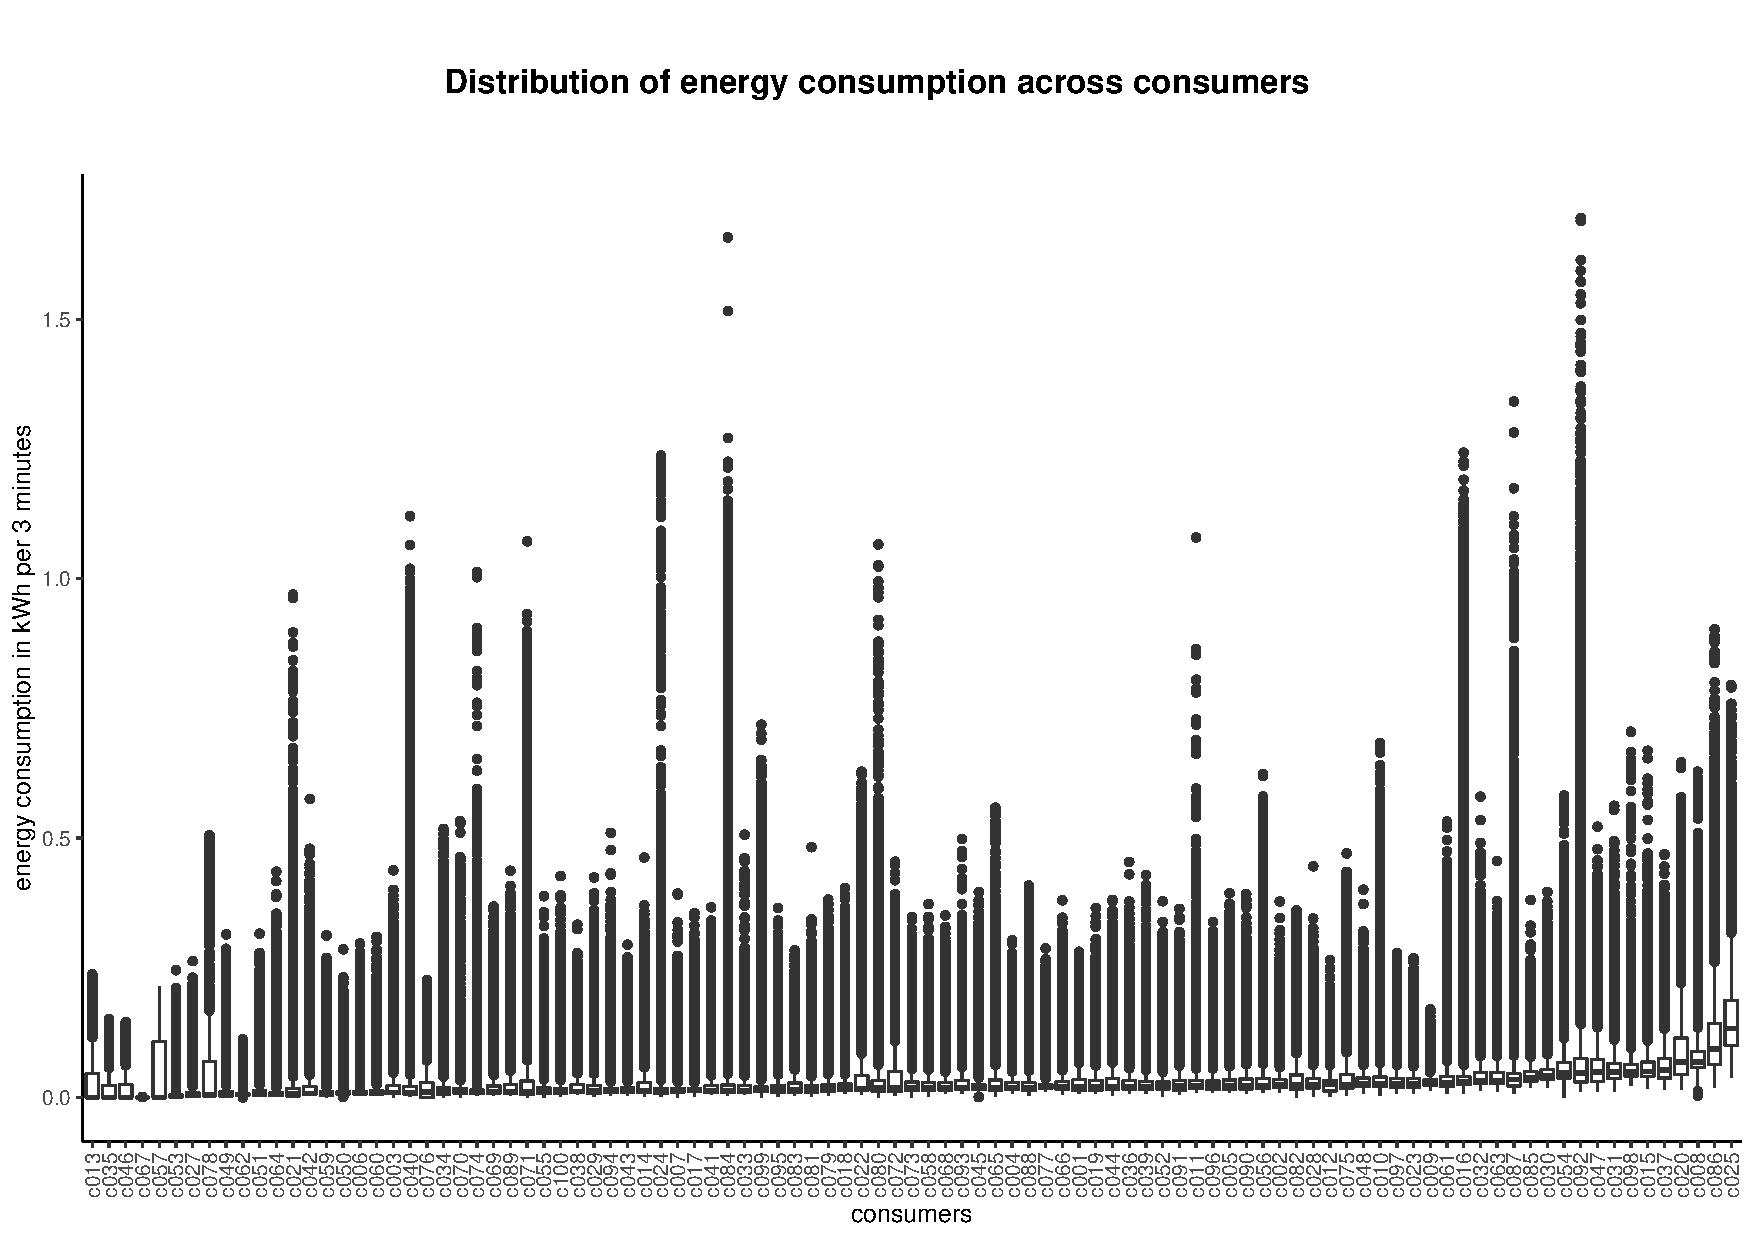
\includegraphics[width=\textwidth]{thesis/graphs/consumer_boxplots_consumption.jpg}
\caption[Boxplots of each consumer's energy consumption in kWh/3-minutes interval]{Boxplots of each consumer's energy consumption in kWh per 3-minutes interval. Ordered by increasing median consumption per 3-minutes interval. \quantnet\href{https://github.com/QuantLet/BLEM/tree/master/BLEMdescStatEnergyData}{BLEMdescStatEnergyData}}
\label{Fig:cons_boxplots_consumption}
\end{figure}



%%%%%%%%%%%
\newpage
\subsubsection{Prosumer data sets}

Interestingly, the prosumer data sets show very different consumption patterns than the pure consumer data sets. This may be due to the fact, that the recorded energy consumption per 3-minutes interval is the net value of the actual energy consumption minus the energy production in the same interval. For example, if prosumer~024's recorded consumption value is 0.021 kWh in the time period from 13.05.2017~06:03 to 06:06, and its energy production in the same interval is 0.018 kWh (which is not recorded and therefore not known), its actual energy consumption in that time interval is 0.039 kWh. However, this actual energy consumption is unknown as the energy production per 3-minutes interval is not recorded. Only a surplus of energy production over consumption would be recorded as an increase in the energy out readings (see Table~\ref{Tab:p089}).

Visual inspection of the consumption time series of the prosumer data sets already reveals that the consumption patterns in most cases do not resemble the consumer households' consumption patterns. Figure~\ref{Fig:prosenergycons_peculiar} shows the consumption values of four prosumers that exemplify four types of generalized consumption patterns that can be found in the prosumer data.
%
\begin{sidewaysfigure}[htbp]
    \centering
    \begin{minipage}[h]{\dimexpr.5\textheight-0.15em}
    \includegraphics[width=\textwidth]{thesis/graphs/timeseries/p004_cons.pdf}
    \end{minipage}
    \begin{minipage}[h]{\dimexpr.5\textheight-0.15em}
    \includegraphics[width=\textwidth]{thesis/graphs/timeseries/p050_cons.pdf}
    \end{minipage}\\
    
    \begin{minipage}[h]{\dimexpr.5\textheight-0.15em}
    \includegraphics[width=\textwidth]{thesis/graphs/timeseries/p061_cons.pdf}
    \end{minipage}
    \begin{minipage}[h]{\dimexpr.5\textheight-0.15em}
    \includegraphics[width=\textwidth]{thesis/graphs/timeseries/p093_cons.pdf}
    \end{minipage}
    
    \caption[Examples for types of prosumer energy consumption patterns]{Exemplary prosumers representing different types of prosumer energy consumption patterns. \quantnet\href{https://github.com/QuantLet/BLEM/tree/master/BLEMplotEnergyData}{BLEMplotEnergyData}}
    \label{Fig:prosenergycons_peculiar}
\end{sidewaysfigure}

\noindent These four generalized types of consumption patterns are: (1) The net energy consumption of the prosumer is zero at night, starts to increase at around 6 a.m., fluctuates over daytime, and decreases to zero again at around 6 p.m.~(see exemplary prosumer 004 in Figure~\ref{Fig:prosenergycons_peculiar}). (2) The net energy consumption is mostly non-zero and fluctuates (in a regular pattern) at low levels with occasional net consumption spikes (see exemplary prosumer 050 in Figure~\ref{Fig:prosenergycons_peculiar}). This is the most generic type of prosumer energy consumption patterns. (3) The net consumption is zero for most of the year (see exemplary prosumer 061 in Figure~\ref{Fig:prosenergycons_peculiar}). This may be due to a surplus in net energy production. (4) The net energy consumption is mostly non-zero, fluctuates very little at a relatively high level (see exemplary prosumer 093 in Figure~\ref{Fig:prosenergycons_peculiar}), and the net energy consumption drops only occasional from this high level. Type (1) and (2) represent the majority of data sets. Type (1) is very easily identifiable and represents 30~\% of the data sets. Type (2) is more generic, and therefore, comprises more heterogenic patterns with 56~\% of the data sets belonging to this type. Type (3) and (4), exemplary shown in the lower two panels of Figure~\ref{Fig:prosenergycons_peculiar}, only represent a minority of the data sets.

Overall, it becomes clear that the net energy consumption of prosumers may exhibit very different patterns than the energy consumption of consumers. This exacerbates the prediction task for prosumers significantly. Furthermore, the total consumption of prosumers follows a very different distribution than the total consumption of consumers (see Figure~\ref{Fig:pros_total_consumption}). The maximum total net consumption of a prosumer was 424,893 kWh, which is 15 times more than the maximum total consumption of a consumer. 19 out of 100 prosumers net consumed more energy than the biggest consumer household contained in the data. Also, the dispersion of the total net consumption is much higher with an IQR of 22,149 kWh for prosumers' total net consumption compared to an IQR of 2,542 kWh for consumers' total consumption in 2017.

\begin{figure}[H]
 \centering
\includegraphics[width=\textwidth]{thesis/graphs/prosumer_totalconsumption.pdf}
\caption[Prosumers’ total energy consumption in 2017]{Prosumers’ total energy consumption (in kWh) in 2017 ordered from high to low. \quantnet\href{https://github.com/QuantLet/BLEM/tree/master/BLEMdescStatEnergyData}{BLEMdescStatEnergyData}}
\label{Fig:pros_total_consumption}
\end{figure}

Finally, Figure~\ref{Fig:pros_boxplots_consumption} offers another perspective on the heterogeneity of the prosumer data sets. The figure shows a boxplot for each prosumer's energy consumption values per 3-minutes interval. The prosumers are sorted on the x-axis by their median net energy consumption. As can be seen here, while the median for the majority of the prosumers is relatively close to zero, the IQR and the total range of net consumption values differ substantially between prosumers. Approximately the same range of net consumption values per 3-minutes interval can be accompanied by a median of 0.0003 kWh or by a median of 1.9110 kWh (compare p088 and p094 in Figure~\ref{Fig:pros_boxplots_consumption}).

\begin{figure}[ht]
 \centering
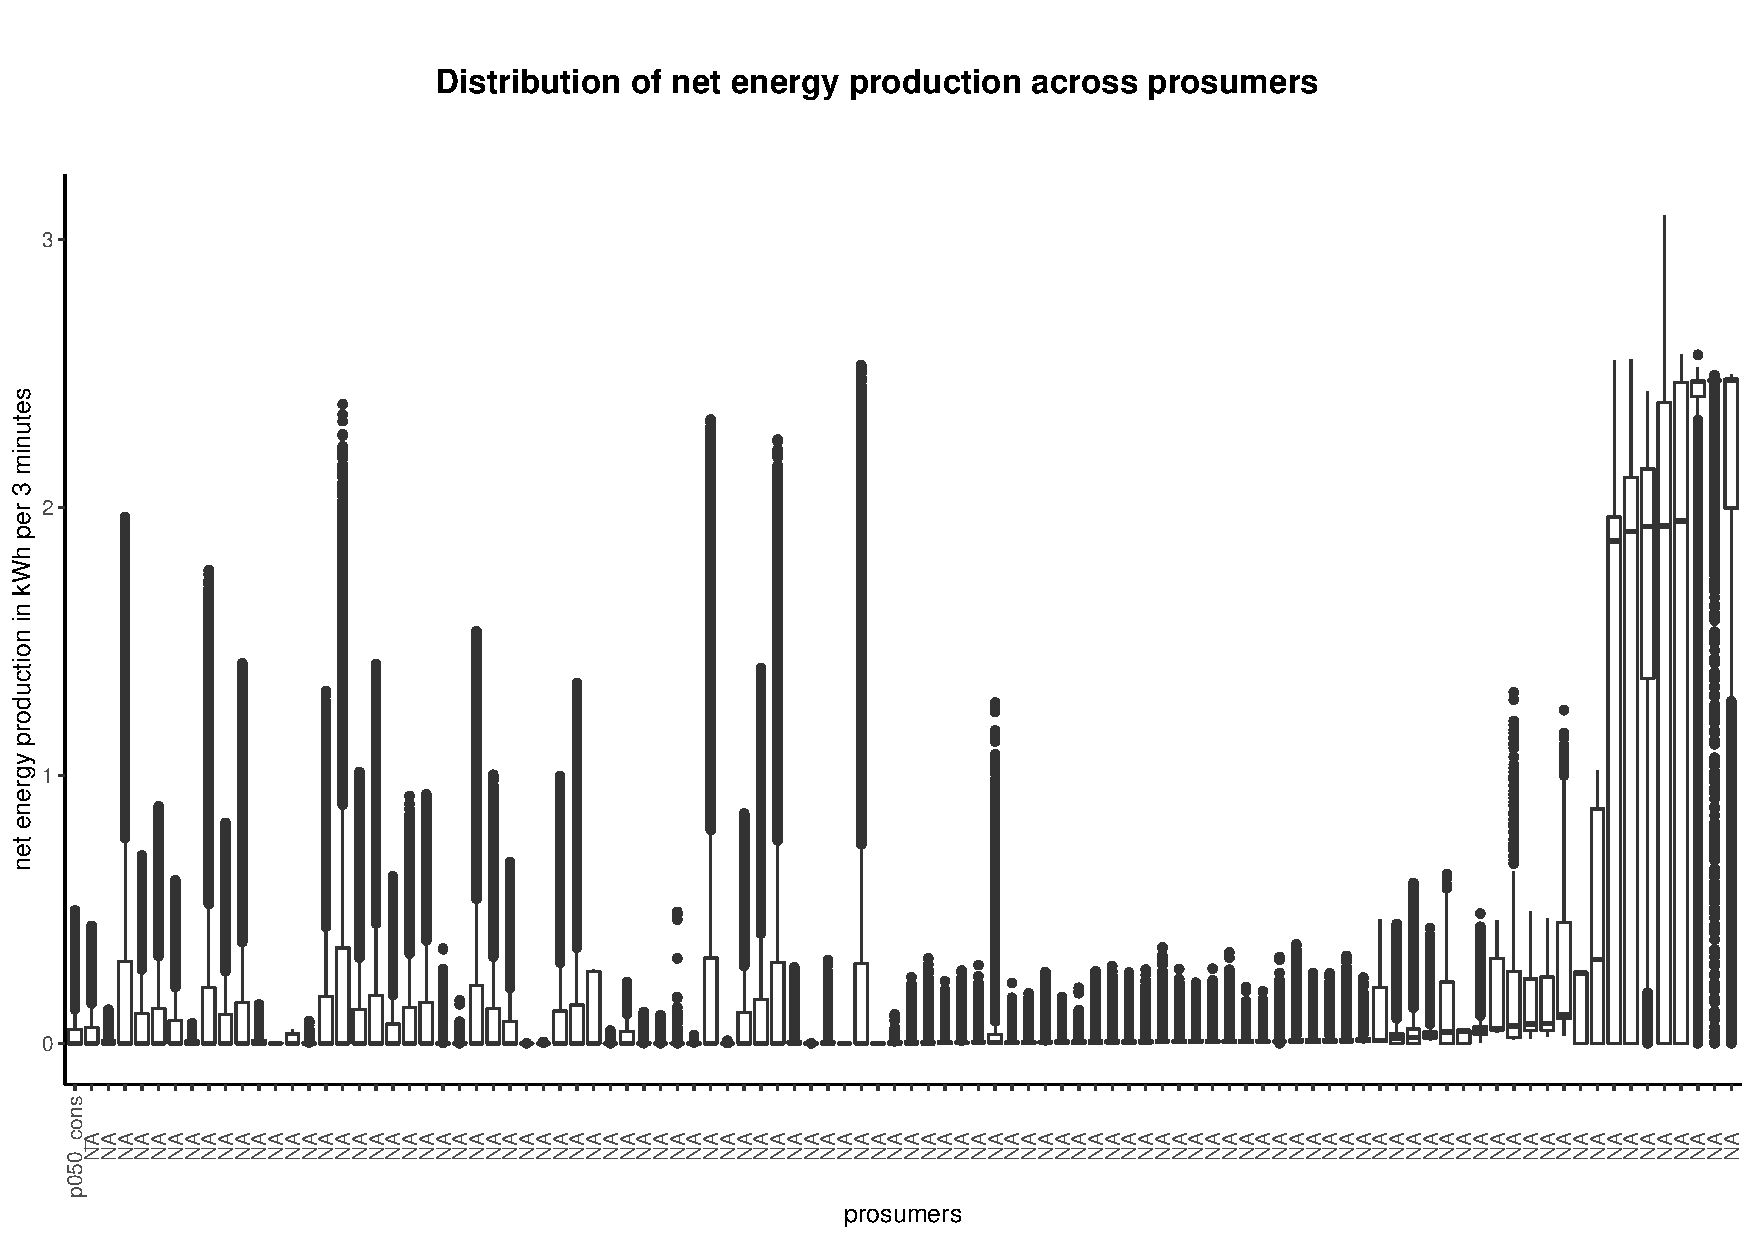
\includegraphics[width=\textwidth]{thesis/graphs/prosumer_boxplots_consumption.jpg}
\caption[Boxplots of each prosumer's net energy consumption in kWh/3-minutes interval]{Boxplots of each prosumer's net energy consumption in kWh per 3-minutes interval. Ordered by increasing median consumption per 3-minutes interval. \quantnet\href{https://github.com/QuantLet/BLEM/tree/master/BLEMdescStatEnergyData}{BLEMdescStatEnergyData}}
\label{Fig:pros_boxplots_consumption}
\end{figure}

Prosumers are defined by the fact, that they not only consume energy but also produce energy -- primarily for their own consumption. However, any surplus in energy production over energy consumption is fed into the grid, and thus, recorded by the smart meter as an increase in the energy out readings. As explained above, these energy out readings are used to compute the net energy production per 3-minutes interval by first-differencing. Surprisingly, only 14 out of 100 available prosumer data sets contained non-zero net energy production values at all. This becomes clear when looking at Figure~\ref{Fig:pros_total_production}, which shows the total net energy production of all prosumers. 86 of those prosumers fed zero kWh into the grid during 2017. The top three net energy producing prosumers, however, fed a total of 1,259,686 kWh into the grid, which is more than twice the amount all 100 consumer households consumed together\footnote{Cumulatively, the 100 consumer households, for which data is available, consumed 559,369 kWh in 2017.}. For comparison, a typical photovoltaic installation on a private residential building with a roof surface area of 150 m$^2$ produces approximately 20,000 kWh per year \citep{energieatlas:2018}.

\begin{figure}[htbp]
 \centering
\includegraphics[width=\textwidth]{thesis/graphs/prosumer_totalproduction.pdf}
\caption[Prosumers’ total energy production in 2017]{Prosumers’ total energy production (in kWh) in 2017 ordered from high to low. \quantnet\href{https://github.com/QuantLet/BLEM/tree/master/BLEMdescStatEnergyData}{BLEMdescStatEnergyData}}
\label{Fig:pros_total_production}
\end{figure}

Prosumer~026, for example, has a relatively low total net energy production. However, its net energy production pattern looks like a typical household with a photovoltaic installation (see Figure~\ref{Fig:energyconsprod_p026p086}). The net energy consumption is (almost) always zero, while the net energy production on most days rather smoothly increases and decreases throughout the day with occasional drops, probably caused by changes in the cloud cover. Furthermore, the net energy production increases in the summer months and decreases notably in winter.

Compare this to prosumer~086 that has a stable, very high net energy production over the whole course of 2017. There are only a few drops, which are accompanied by a simultaneous net energy consumption (visible by the small blue spikes in the upper panel of the right graph of Figure~\ref{Fig:energyconsprod_p026p086}, whenever the net production drops). Note also the different scales of the y-axis. The net production of prosumer 086 is in the range of 1 kWh per 3-minutes interval while the net production of prosumer~026 barely surpasses 0.4 kWh per 3-minutes interval.
%
\begin{sidewaysfigure}[htbp]
\centering
\begin{minipage}[h]{\dimexpr.5\textwidth-0.15em}
\includegraphics[width=\textwidth]{thesis/graphs/timeseries/p026_prod&cons.pdf}
\end{minipage}
\begin{minipage}[h]{\dimexpr.5\textheight-0.15em}
\includegraphics[width=\textwidth]{thesis/graphs/timeseries/p086_prod&cons.pdf}
\end{minipage}

\caption[Energy consumption and production recordings of prosumer~026 and 086]{Energy consumption and production recordings of prosumer~026 and 086. The first panel in the respective graph shows the full year 2017, the second panel zooms in to one month (May), and the third panel zooms in to one day (May, 13). \quantnet\href{https://github.com/QuantLet/BLEM/tree/master/BLEMplotEnergyData}{BLEMplotEnergyData}}
\label{Fig:energyconsprod_p026p086}

\end{sidewaysfigure}
%
A plausible explanation for the net production pattern exhibited by prosumer~086 may be a combined heat and power unit (CHP, also called block-type thermal power station or BTTP). This assumption is also supported by the increasing frequency of drops in net energy production over the summer months. In these months much less heating is needed resulting in more downtime of the CHP and therefore also more periods of zero net energy production. However, as mentioned in the discussion of the consumer data sets, unfortunately, there is no additional context information available for the data sets at hand making this kind of assumption purely speculative.

In conclusion, it becomes clear that the prosumers' net energy consumption and production follow much less easily explainable patterns. The net energy consumption is much more heterogeneous. Additionally, most prosumer data sets do not contain any recordings of net energy production at all. Of those prosumers that do have positive net production values, most surpass the energy consumption of a typical household with their net energy production by far. What these findings imply for the suitability of the data sets for the prediction task at hand will be discussed in Section~\ref{Sec:Data;Subsec:Exclusion}.



%%%%%%%%%%%%%%%%%%%%%%%%%%%%%%%%%%%%%
%%%   Peculiarities in the data   %%%
%%%%%%%%%%%%%%%%%%%%%%%%%%%%%%%%%%%%%

\subsection{Peculiarities in the data}\label{Sec:Data;Subsec:Peculiarities}



%%%%%%%%%%%
\subsubsection{Consumer data sets}

The data sets were analyzed for peculiarities in the time series patterns that seemed to be systematically different from the majority of the data sets. One such peculiarity is the occurrence of zero values. In any household that does not produce its own energy (pure consumer household), energy consumption of 0 kWh, even only for a very short period of time, seems to be very unlikely (apart from the rare case of a power outage in the area or when the main switch of the household is turned off). Thus, it is not surprising that 93~\% of the data sets do not contain any 0 kWh measurements per 3-minutes interval at all. Of the remaining 6 data sets, one contains just a single measurement of 0 kWh, which seems plausible. The other data set with a small amount of zero values is consumer~082 which was discussed in detail in Section~\ref{Sec:Data;Subsec:Description}. In Figure~\ref{Fig:energycons_c082} showing consumer~082's consumption values, it is visible that although the consumption pattern does not change substantially, the lowest values of the daily fluctuations are lower in the second half of 2017 than in the first half. However, this seems still a plausible consumption pattern for a typical household. The other five data sets, on the contrary, contain between 34~\% and 54~\% of zero values. Examining the consumption time series more closely also reveals, that these households exhibit a systematically different consumption pattern than one would expect from a typical household.

Figure~\ref{Fig:consenergycons_peculiar} shows the time series of the aforementioned four consumers with a high share of zero measurements. Consumer~013 and 035, both, show a very similar pattern of daily energy consumption. Looking at the middle panel of the two upper graphs in Figure~\ref{Fig:consenergycons_peculiar}, the regularity of the consumption increases and decreases on each day is striking. The lower panel shows again, exemplary, May 13, 2017. Energy consumption starts to (almost linearly) increase at about 6~a.m.~and decreases to 0 kWh at about 6 p.m. This also explains the share of 53~\% and 54~\% of zero values in those two data sets: Almost exactly 12 hours per day (from midnight to 6 a.m.~and from 6 p.m.~to midnight) the consumption is zero, while the energy consumption fluctuates in the meantime with a relatively high ``base" consumption. Switching back to the middle panel, it is noticeable that there are some days in May with an even smoother energy consumption increase and decrease over the course of the day. As there is no further socio-demographic data available, it can be only guessed what the reason for such different consumption patterns are. The most likely explanation seems to be that the consumption time series of consumer~013 and consumer~035 belong to small businesses rather than to households.

\begin{sidewaysfigure}[htbp]
    \centering
    \begin{minipage}[ht]{\dimexpr.5\textheight-0.15em}
    \includegraphics[width=\textwidth]{thesis/graphs/timeseries/c013_cons.pdf}
    \end{minipage}
    \begin{minipage}[ht]{\dimexpr.5\textheight-0.15em}
    \includegraphics[width=\textwidth]{thesis/graphs/timeseries/c035_cons.pdf}
    \end{minipage}\\
    
    \begin{minipage}[ht]{\dimexpr.5\textheight-0.15em}
    \includegraphics[width=\textwidth]{thesis/graphs/timeseries/c067_cons.pdf}
    \end{minipage}
    \begin{minipage}[ht]{\dimexpr.5\textheight-0.15em}
    \includegraphics[width=\textwidth]{thesis/graphs/timeseries/c076_cons.pdf}
    \end{minipage}
    
    \caption[Energy consumption of consumers with conspicuous consumption patterns]{Energy consumption recordings of consumers with conspicuous consumption patterns. \quantnet\href{https://github.com/QuantLet/BLEM/tree/master/BLEMplotEnergyData}{BLEMplotEnergyData}}
    \label{Fig:consenergycons_peculiar}
\end{sidewaysfigure}

The lower two graphs of Figure~\ref{Fig:consenergycons_peculiar} show the energy consumption time series of consumer~067 and consumer~076. Consumer~067's consumption pattern zoomed in to one month (middle panel) rather looks like an electrocardiogram than what one would expect from a household energy consumption time series. The regularity of frequency and amplitude is obvious but not easily explained. Consumers~076's consumption pattern looks less suspicious at first sight. However, closer inspection reveals the same daily pattern of increasing consumption throughout the day and very low to zero energy consumption at night. This, again, rather resembles the energy consumption pattern of a business building or office rooms than a typical household.



%%%%%%%%%%%
\newpage
\subsubsection{Prosumer data sets}

For prosumers, peculiarities in the time series pattern can be found either in the net energy consumption or net energy production or in combination. As net energy consumption is much more heterogeneous in the prosumer data sets than in the consumer data sets, it is less obvious what patterns fall outside the norm. However, some prosumers still exhibit obvious anomalies in their consumption patterns. Prosumers~046, 061, and 079 stand out as their consumption is zero for the largest part of the year. This would be an expected pattern if they were net energy producers during this time period. However, as they do not feed in any produced energy at all in 2017, this consumption pattern indicates a data problem. Prosumer~038 attracts attention by having a very low total net energy consumption of just 18 kWh in 2017 and zero net production. Moreover, this energy is consumed at an extremely low level of around 0.0001 kWh with a standard deviation of $\sigma=2\times10^{-6}$ and just one single drop from this level to zero in the whole year (see Figure~\ref{Fig:energycons_p038}).
%
\begin{figure}[!htb]
 \centering
\includegraphics[width=\textwidth]{thesis/graphs/timeseries/p038_cons.pdf}
\caption[Energy consumption recordings of prosumer 038]{Energy consumption recordings of prosumer~038. The first panel shows the full year 2017, the second panel zooms in to one month (May), and the third panel zooms in to one day (May, 13). \quantnet\href{https://github.com/QuantLet/BLEM/tree/master/BLEMplotEnergyData}{BLEMplotEnergyData}}
\label{Fig:energycons_p038}
\end{figure}
%
Six more prosumers exhibit a similar pattern of stable net energy consumption level with occasional drops to zero but no spikes above this stable level. None of them is a net energy producer at any time.
  
Lastly, prosumer~019 is worth mentioning as it is the only prosumer data set that records a total net energy consumption of 0 kWh for 2017. As the net energy production, however, contains a substantial amount of zero values as well, it seems implausible that prosumer 019 is a regular household. For a household, it appears unlikely that the energy consumption is always zero when the energy production is zero as well.

Regarding the production time series, most of the prosumer data sets are peculiar in so far as they have only zero net production values. It seems at least somewhat unlikely that a majority of households equipped with energy production capacities consumes more than it produces over the whole course of the year at any point in time. However, it was unfortunately not possible to get feedback from Discovergy due to privacy and internal policy reasons on why 84 out of 100 prosumer data sets did not record any electricity fed into the grid at all. Of the remaining 14 data sets, prosumer 084 and 085 stand out as their net energy production time series is almost a flat line at 2.5 kWh per 3-minutes interval. Their graphs are shown in Figure~\ref{Fig:energyconsprod_p084p085}.

\begin{sidewaysfigure}[htbp]
\centering
\includegraphics[width=.5\textwidth-0.15em]{thesis/graphs/timeseries/p084_prod&cons.pdf}
\includegraphics[width=.5\textwidth-0.15em]{thesis/graphs/timeseries/p085_prod&cons.pdf}

\caption[Energy consumption and production recordings of prosumer 084 and 085]{Energy consumption and production recordings of prosumer~084 and 085. The first panel in the respective graph shows the full year 2017, the second panel zooms in to one month (May), and the third panel zooms in to one day (May, 13). \quantnet\href{https://github.com/QuantLet/BLEM/tree/master/BLEMplotEnergyData}{BLEMplotEnergyData}}
\label{Fig:energyconsprod_p084p085}
\end{sidewaysfigure}

In conclusion, it seems like the majority of prosumer data sets with non-zero net production values were recorded by smart meters that just record the energy production of a certain installation and not of a household with production capacity. This is not per se a problem, as these installations can act as a individual agent on a LEM. Even though, they might belong to a household with a separate smart meter, they can sell energy through their own smart meter while the related household's smart meter buys energy. If both smart meters are connected to the same blockchain wallet, this automatically solves the challenge of pricing the energy relative to the own consumption.



%%%%%%%%%%%%%%%%%%%%%%%%%%%%%%
%%%   Data sets excluded   %%%
%%%%%%%%%%%%%%%%%%%%%%%%%%%%%%

\newpage
\subsection{Data sets excluded}\label{Sec:Data;Subsec:Exclusion}
The data sets of consumers~013, 035, 067 and 076 (shown in Figure~\ref{Fig:consenergycons_peculiar}) where excluded from the prediction task. These four consumers plus one additional consumer (consumer~082) exhibited non-negligible shares of zero consumption values leading to their exclusion. Additionally, consumer~046 was excluded as the consumption time series was flat for the most part of 2017. After some initial fluctuations in the first quarter, all fluctuations stopped entirely. Four more consumers were excluded due to conspicuous regularity in daily or weekly consumption patterns. Lastly, consumer~080 was excluded due to very low and stable consumption values with very rare, extreme spikes. The time series graphs of all additionally to the ones shown in Figure~\ref{Fig:consenergycons_peculiar} excluded consumer data sets are shown in Appendix~\hyperlink{AppA1:Figures:Excludedc}{A1}. Consumer~026 was excluded not due to peculiarities in the consumption patterns but due to missing data. For some unknown reason, the last recorded measurement for consumer~026 was 29.12.2017~07:03. As the inclusion of this shorter time series would have lead to difficulties in the forecasting algorithms, this data set was excluded as well.

Out of the 100 prosumer data sets, 86 were excluded from the prediction task due to zero total net energy production in 2017. These ``prosumers" would not act as prosumers in a LEM as they would never actually supply a production surplus to the market. Of the remaining 14 prosumer data sets, prosumer 012 was excluded as the total net energy it fed into the grid in 2017 was just 22 kWh. Even though, the feed-in occurred continuously over the whole year, it never exceeded 0.0013 kWh per 3-minutes interval with a mean of 0.0001 kWh, which is too small to be relevant. Prosumer 015 was excluded as it only fed energy into the grid in the period from 06.01.2017 to 19.01.2017. For all other measurement points the net energy production was zero. The time series graph of the two excluded prosumer data sets with production data are shown in Appendix~\hyperlink{AppA2:Figures:Excludedp}{A2}.

Hence, 88 consumer and 12 prosumer data sets remained for the prediction task. All data sets included a timestamp and the consumption time series for consumers respectively the production time series for prosumers with a total of 175,200 data points each.

%%%%%%%%%%%%%%%%%%%%%%%%%%%%%%%%%%%%%%%%%%%%%%%%%%%%%%%%%%%%%%%%%


\section{Results}\label{Sec:Results}

The results are presented in three parts that correspond to the three research questions put forward in Section~\ref{Sec:Intro;Subsec:Present}: First, the forecasting accuracy of the prediction models is evaluated and reported. Second, the results of the market simulation -- which was run once with the true consumption and production values and once with predicted consumption values in three different supply scenarios -- are presented. Third, the implications of the results of the market simulation are discussed.


%%%%%%%%%%%%%%%%%%%%%%%%%%%%
%%%   Benchmark models   %%%
%%%%%%%%%%%%%%%%%%%%%%%%%%%%

\subsection{Evaluation of the prediction models}\label{Sec:Results;Subsec:Forecast}

Three prediction methods were used to forecast the energy consumption of 88 consumer households and to forecast the energy production of 12 prosumer households 15 minutes ahead: a benchmark model (see Section~\ref{Sec:Method;Subsec:Benchmark}), a LSTM RNN model (see Section~\ref{Sec:Method;Subsec:LSTM}), and a LASSO model (see Section~\ref{Sec:Method;Subsec:LASSO}). All three prediction models were compared and evaluated using the error measures presented in Section~\ref{Sec:Method;Subsec:Error}.


%%%%%%%%%%%
\subsubsection{Consumption data}

The performance of the prediction models was tested on a quarter of the available data. That is, the prediction models were fitted on the consumption values from 01.01.2017~00:00 to 30.09.2017~00:00 which is equivalent to 131,040 data points per data set. For all 88 consumer data sets, the models were fitted separately resulting in as many distinct LASSO and LSTM prediction models. The fitted models were then used to make energy consumption predictions in 15-minutes intervals for each household individually on the data from 01.10.2017~00:00 to 01.01.2018~00:00. This equates to 8,836 predicted values per data set per prediction method.

Figure~\ref{Fig:glimpse_predcons} exemplary shows the true and predicted consumption values of consumer~011 on October 27, 2017. The na\"ive benchmark model just follows the true consumption shifted by one time step (i.e., 15 minutes). This fits the true values generally good, as long as there are no sudden jumps in the household's energy consumption. Spikes in energy consumption, as in this example one occurred in the 15 minutes before 07:30 a.m.~and 08.30 a.m.~respectively, necessarily lead to two periods with high errors of the na\"ive predictor: First, once the jump to a high consumption level occurs and the na\"ive predictor remains at the previous low level, and second, once the consumption suddenly returns to the low consumption level and the na\"ive predictor persists at the high level of the previous period. In such situations, the LASSO and LSTM models are more accurate. Even though they underestimate the jumps in energy consumption, they do not lag behind as much as the na\"ive predictor and, generally, have the ability to anticipate movements. However, the exemplary glimpse onto the predicted consumption values of consumer~011 already reveals that also the sophisticated prediction models lack the ability to accurately predict sudden movements in the energy consumption and tend to overestimate low consumption levels and underestimate spikes in energy consumption.
%
\begin{figure}[htbp]
    \centering
    \includegraphics[width=\textwidth]{thesis/graphs/evaluation/c011_pred_cons.pdf}
    \caption[Exemplary 24 hours of true and predicted consumption values]{Exemplary 24 hours of true and predicted consumption values of consumer 011. \quantnet\href{https://github.com/QuantLet/BLEM/tree/master/BLEMplotEnergyPreds}{BLEMplotEnergyPreds}}
    \label{Fig:glimpse_predcons}
\end{figure}
%

Systematically analyzing the total over- and underestimation of the different prediction models on each consumer data set confirms this impression. Figure~\ref{Fig:overunderestimation} displays the total sum of over- and underestimation errors of each prediction method per data set. As one would expect, the na\"ive benchmark model consistently over- and underestimated by the same amount per data set. The reason for that is that the sum of over- and underestimation errors only depends on the amplitude of the spikes in energy consumption. Thus, overestimation errors occur in the same frequency and magnitude as underestimation errors. The LASSO model achieved overall lower total sums of errors than the benchmark model. Notably, the sum of underestimation errors is higher across the data sets than the sum of overestimation errors. This points towards a general tendency of underestimating sudden increases in energy consumption by the LASSO model.
%
\begin{figure}[htbp]
    \centering
    \includegraphics[width=\textwidth]{thesis/graphs/evaluation/c_barplot_naive_overunderestimation.pdf}\\\vspace{.6cm}
    \includegraphics[width=\textwidth]{thesis/graphs/evaluation/c_barplot_LASSO_overunderestimation.pdf}\\\vspace{.6cm}
    \includegraphics[width=\textwidth]{thesis/graphs/evaluation/c_barplot_LSTM_overunderestimation.pdf}
    \caption[Sum of total over- and underestimation errors per consumer data set]{Sum of total over- and underestimation errors of energy consumption per consumer data set and prediction model. \quantnet\href{https://github.com/QuantLet/BLEM/tree/master/BLEMplotPredErrors}{BLEMplotPredErrors}}
    \label{Fig:overunderestimation}
\end{figure}
%

\noindent The LSTM model on the other hand shows a much higher variability in the sums of over- and underestimation errors. By tendency, the overestimation errors of the LSTM model were smaller than those of the LASSO and benchmark models. Nevertheless, the underestimation is much more pronounced in the case of the LSTM model. Especially, some data sets stand out regarding the high sum of underestimation errors. This points towards a much higher heterogeneity in the suitability of the LSTM model to predict consumption values depending on the energy consumption pattern of the specific data set. The LASSO model on the other hand seems to be more equally well suited for all data sets and their particular consumption patterns.


The average performance of the three prediction models across all 88 data sets is shown in Table~\ref{Tab:avg_errormeasures}. As can be seen, LASSO and LSTM consistently outperformed the benchmark model according to MAE, RMSE, MAPE, and MASE\footnote{Note that the MASE score of the benchmark model must be exactly 1 as the MASE is defined as the mean absolute error relative to the MAE of the na\"ive predictor (see Equation~\ref{Eq:naivepred}).}. Interestingly, due to the heavy penalty NRMSE puts on comparably large prediction errors, both sophisticated prediction methods perform worse according to NRMSE, however.
%
\begingroup\catcode`"=9
\begin{table}[ht]
{\footnotesize
    \csvreader[centered tabular=l|SSSSS,
    before reading=\sisetup{round-mode=places,round-precision=2,round-integer-to-decimal},
    filter not strcmp={\thecsvinputline}{1},
    table head=
    \hline\hline
     \multicolumn{1} {l}{\textbf{Model}} & \multicolumn{1} {c}{\textbf{MAE}} & \multicolumn{1} {c}{\textbf{RMSE}} & \multicolumn{1} {c}{\textbf{MAPE}} & \multicolumn{1} {c}{\textbf{NRMSE}} & \multicolumn{1} {c}{\textbf{MASE}}\\
    \hline,
    no head,
    separator=comma,
    respect all,
    late after line=\\,
    table foot=\hline \hline]
    {thesis/tables/avg_errorMeasures_c.csv}{}%
    {\csvcolii & \csvcoliii & \csvcoliv & \csvcolv & \csvcolvi & \csvcolvii}}%
    \caption[Mean of error measures for prediction on consumer data sets]{Mean of error measures for the prediction of energy consumption across all 88 consumer data sets. \quantnet\href{https://github.com/QuantLet/BLEM/tree/master/BLEMevaluateEnergyPreds}{BLEMevaluateEnergyPreds}}
    \label{Tab:avg_errormeasures}
\end{table}
\endgroup
%

A detailed analysis of this unexpected result reveals that it is mainly driven by an extremely bad NRMSE score for LSTM and LASSO on merely one out of the 88 data sets. As can be seen in Figure~\ref{Fig:heatmaps}, the predictions on consumer data set 027 have a particularly high NRMSE (and MAPE) compared to all other data sets. However, this pattern is not present in the absolute error measures. Further investigating the prediction errors of the forecasts on consumer 027 exposes that the high NRMSE score is driven by merely one observations: Between 24.11.2017 11:30 and 11:45 the energy consumption falls below 3 $\times$ $10^{-6}$. Due to this true value, $x_t$, which is very close to zero, the relative squared error $e_t = \left(\frac{\widehat{x}_t-x_t}{x_t}\right)^2$ is extremely high (see Appendix~\hyperlink{AppA4:Figures:erroranalysis}{A4}). This single extreme relative error pushes the NRMSE of the LSTM predictions to the staggering value of $\text{NRMSE}_{c027}=2383.46$. The same is true for MAPE, although not as extreme.
%
\begin{figure}[ht]
 \centering
 \includegraphics[width=\textwidth]{thesis/graphs/evaluation/c_heatmap_MAE.pdf}
 \includegraphics[width=\textwidth]{thesis/graphs/evaluation/c_heatmap_MAPE.pdf}
 \includegraphics[width=\textwidth]{thesis/graphs/evaluation/c_heatmap_RMSE.pdf}
 \includegraphics[width=\textwidth]{thesis/graphs/evaluation/c_heatmap_NRMSE.pdf}
 \includegraphics[width=\textwidth]{thesis/graphs/evaluation/c_heatmap_MASE.pdf}
\caption[Heatmaps of error measures for prediction of consumption values]{Heatmap of MAE, MAPE, RMSE, NRMSE, and MASE scores for the prediction of consumption values per consumer data set. \quantnet\href{https://github.com/QuantLet/BLEM/tree/master/BLEMevaluateEnergyPreds}{BLEMevaluateEnergyPreds}}
\label{Fig:heatmaps}
\end{figure}
%

Based on this insight, it seemed reasonable to reevaluate the average performance of the prediction methods across all consumer data sets using the median instead of the mean. Calculating the median error measures for all predictions on the consumer data sets eliminates the distortion by outliers. Thus, Table~\ref{Tab:median_errormeasures} shows the same error measures as Table~\ref{Tab:avg_errormeasures} but uses the median instead of the mean to summarize the models performance across all consumer data sets. This shows the LASSO model performed best overall with the lowest median MAE, RMSE, MAPE, NRMSE, and MASE scores. With a median MAPE across the 88 consumer datasets of 17.38~\%, it achieved an even better score in the present research than in the implementation of \citet{Li:2017}, who achieved a score of 20.06~\%.
%
\begingroup\catcode`"=9
\begin{table}[ht]
{\footnotesize
    \csvreader[centered tabular=l|SSSSS,
    before reading=\sisetup{round-mode=places,round-precision=2,round-integer-to-decimal},
    filter not strcmp={\thecsvinputline}{1},
    table head=
    \hline\hline
     \multicolumn{1} {l}{\textbf{Model}} & \multicolumn{1} {c}{\textbf{MAE}} & \multicolumn{1} {c}{\textbf{RMSE}} & \multicolumn{1} {c}{\textbf{MAPE}} & \multicolumn{1} {c}{\textbf{NRMSE}} & \multicolumn{1} {c}{\textbf{MASE}}\\
    \hline,
    no head,
    separator=comma,
    respect all,
    late after line=\\,
    table foot=\hline \hline]
    {thesis/tables/median_errorMeasures.csv}{}%
    {\csvcolii & \csvcoliii & \csvcoliv & \csvcolv & \csvcolvi & \csvcolvii}}%
    \caption[Median of error measures for prediction on consumer data sets]{Median of error measures for the prediction of energy consumption across all 88 consumer data sets. \quantnet\href{https://github.com/QuantLet/BLEM/tree/master/BLEMevaluateEnergyPreds}{BLEMevaluateEnergyPreds}}
    \label{Tab:median_errormeasures}
\end{table}
\endgroup
%

\newpage
The superior performance of the LASSO model is also clearly visible in Figure~\ref{Fig:boxplots_errormeasures}. Additionally noteworthy here are the differences in the IQR of the error measures between the prediction methods. Both, the LASSO as well as the LSTM model, have error measures with a smaller IQR across the consumer data sets than the benchmark model. Furthermore, even though the LASSO error measures consistently have the lowest median of all three prediction models, the IQR of the relative error measures MAPE and NRMSE is very similar between LASSO and LSTM.
%
\begin{figure}
    \centering
    \includegraphics[width=.5\textwidth-5pt]{thesis/graphs/evaluation/c_boxplot_MAE.pdf}
    \includegraphics[width=.5\textwidth-5pt]{thesis/graphs/evaluation/c_boxplot_MAPE.pdf} \\
    
    \includegraphics[width=.5\textwidth-5pt]{thesis/graphs/evaluation/c_boxplot_RMSE.pdf}
    \includegraphics[width=.5\textwidth-5pt]{thesis/graphs/evaluation/c_boxplot_NRMSE.pdf} \\
    \caption[Boxplots of error measures for prediction of consumption values]{Boxplots of MAE, MAPE, RMSE, and NRMSE scores across 88 consumer data sets for the three different prediction models (the upper 3~\%-quantile of the error measures is cut off for better readability). \quantnet\href{https://github.com/QuantLet/BLEM/tree/master/BLEMevaluateEnergyPreds}{BLEMevaluateEnergyPreds}}
    \label{Fig:boxplots_errormeasures}
\end{figure}
%

Interestingly, there are some consumer data sets which exhibit apparently much harder to predict consumption patterns than the other data sets. This is exemplified by the outliers of the MAPE and NRMSE boxplots, and also, by the heatmaps displayed in Figure~\ref{Fig:heatmaps}. Unfortunately, the heatmaps of the relative error measures MAPE and NRMSE are dominated by the very high values for consumer 027. An alternative way to calculate those error measures according to \citet{Hyndman:2006} to avoid very skewed NRMSE or MAPE distribution in the presence of values close to zero is to use the median instead of the mean error. Thus, the mean absolute percentage error becomes the median absolute percentage error (MdAPE) and the normalized root mean squared error becomes the normalized root median squared error (NRMdSE). Taking consumer 027 as an example, the difference becomes clear: The normalized root mean squared error is $\text{NRMSE}_{c027}=2383.46$, while the normalized root \emph{median} squared error is only $\text{NRMdSE}_{c027}=33.43$ (which is still comparatively high). The same holds true for MAPE and MdAPE\footnote{The average MdAPE and NRMdSE across all consumer data sets in comparison to MAPE and NRMSE are presented in Appendix~\hyperlink{AppB2:Tables:avg_errM_wMedian}{B2}.}. Accordingly, the heatmaps for MdAPE and NRMdSE are shown in Figure~\ref{Fig:heatmaps_median}. They confirm that there is a wide variation in the performance of the same prediction methods on the same kind of data but from different households. Therefore one can conclude, that apparently, there is no ``one-size-fits-all'' approach for households' very short-term energy consumption forecasting.

Nevertheless, it is obvious that the LASSO model performed best overall. Hence, the predictions on the last quarter of the data produced by the fitted LASSO model for each consumer data set will be used for the evaluation of the following market simulation.
%
\begin{figure}[ht]
 \centering
 \includegraphics[width=\textwidth]{thesis/graphs/evaluation/c_heatmap_MdAPE.pdf}
 \includegraphics[width=\textwidth]{thesis/graphs/evaluation/c_heatmap_NRMdSE.pdf}
\caption[Heatmaps of MdAPE and NRMdSE for consumption values]{Heatmap of MdAPE and NRMdSE scores for the prediction of consumption values per consumer data set. \quantnet\href{https://github.com/QuantLet/BLEM/tree/master/BLEMevaluateEnergyPreds}{BLEMevaluateEnergyPreds}}
\label{Fig:heatmaps_median}
\end{figure}
%



%%%%%%%%%%%
\subsubsection{Production data}

Also for the production data, the performance of the prediction models was tested on a quarter of the production time series. That is, the prediction models were fitted on the production values from 01.01.2017~00:00 to 30.09.2017~00:00 which is equivalent to 131,040 data points per data set. For all 12 prosumer data sets, the models were fitted separately resulting in as many distinct LASSO and LSTM prediction models. The fitted models were then used to make energy production predictions in 15-minutes intervals for each household individually on the data from 01.10.2017~00:00 to 01.01.2018~00:00. This equates to 8,836 predicted values per data set per prediction method.

Figure~\ref{Fig:glimpse_predprod} exemplary shows the true and predicted production values of prosumer 024 on December 23, 2017. The na\"ive benchmark model just follows the true production shifted by one time step (i.e., 15 minutes). As in the consumption predictions, this fits the true values generally good, as long as there are no sudden spikes in the household's energy production. Spikes or sudden drops in energy production -- as in this example one occurred in the 15 minutes before 06:00 a.m.~-- necessarily lead to a prediction with high error of the na\"ive predictor. In such situations, the LASSO model seems more accurate. Even though, it underestimates the spike in energy production in this example, it does not lag behind as much as the na\"ive predictor and, generally, has the ability to anticipate movements. The LSTM-based predictions, on the contrary, fit even worse than the na\"ive predictor in this example. They almost do not at all follow small movements in the energy production time series and lag behind the true values similarly to the na\"ive predictor. Also, the LSTM model constantly overestimates in periods of zero production and does not follow the upward spike in energy production present in this exemplary snippet of the data.
%
\begin{figure}[htbp]
    \centering
    \includegraphics[width=\textwidth]{thesis/graphs/evaluation/p024_pred_prod.pdf}
    \caption[Exemplary 24 hours of true and predicted production values]{Exemplary 24 hours of true and predicted production values of prosumer 024. \quantnet\href{https://github.com/QuantLet/BLEM/tree/master/BLEMplotEnergyPreds}{BLEMplotEnergyPreds}}
    \label{Fig:glimpse_predprod}
\end{figure}
%

Analyzing the over- and underestimation errors of each prediction method on each producer data set shows the extreme tendency of the LSTM model to underestimate the production values (see Figure~\ref{Fig:overunderestimation_p}). The LSTM's sum of underestimation errors is substantially larger for six out of twelve prosumer data sets and the sum of overestimation is substantially larger for one data set compared to the LASSO and benchmark model. This already indicates a much worse performance of LSTM than LASSO or the na\"ive predictor on the production data.
%
\begin{figure}
    \centering
    \includegraphics[width=.5\textwidth]{thesis/graphs/evaluation/p_barplot_naive_overunderestimation.pdf}\\\vspace{.6cm}
    \includegraphics[width=.5\textwidth]{thesis/graphs/evaluation/p_barplot_LASSO_overunderestimation.pdf}\\\vspace{.6cm}
    \includegraphics[width=.5\textwidth]{thesis/graphs/evaluation/p_barplot_LSTM_overunderestimation.pdf}
    \caption[Sum of total over- and underestimation errors per prosumer data set]{Sum of total over- and underestimation errors of energy production per prosumer data set and prediction model. \quantnet\href{https://github.com/QuantLet/BLEM/tree/master/BLEMplotPredErrors}{BLEMplotPredErrors}}
    \label{Fig:overunderestimation_p}
\end{figure}
%

The first impression is confirmed by the average of the error measures across the 12 prosumer data sets shown in Table~\ref{Tab:avg_errormeasures_p}. The LSTM model on average performs much worse than the LASSO and the benchmark model according to MAE, RMSE, and MASE. Computing the median across the 12 prosumer data sets gives the same qualitative results, although the performance differences are not as extreme (see Appendix~\hyperlink{AppB3:Tables:medain_errM_prod}{B3}). MAPE and NRMSE cannot be computed as all production time series contain zero values\footnote{As can be seen in Equation~\ref{Eq:MAPE} and Equation~\ref{Eq:NRMSE}, MAPE and NRMSE are not defined if the true value $x_t$ equals zero which is why they cannot be computed for the predictions on production data.}.
%
\begingroup\catcode`"=9
\begin{table}[ht]
{\footnotesize
    \csvreader[centered tabular=l|SSS,
    before reading=\sisetup{round-mode=places,round-precision=2,round-integer-to-decimal},
    filter not strcmp={\thecsvinputline}{1},
    table head=
    \hline\hline
     \multicolumn{1} {l}{\textbf{Model}} & \multicolumn{1} {c}{\textbf{MAE}} & \multicolumn{1} {c}{\textbf{RMSE}} & \multicolumn{1} {c}{\textbf{MASE}}\\
    \hline,
    no head,
    separator=comma,
    respect all,
    late after line=\\,
    table foot=\hline \hline]
    {thesis/tables/avg_errorMeasures_p.csv}{}%
    {\csvcolii & \csvcoliii & \csvcoliv & \csvcolv}}%
    \caption[Mean of error measures for prediction on prosumer data sets]{Mean of error measures for the prediction of energy production across all 12 prosumer data sets. \quantnet\href{https://github.com/QuantLet/BLEM/tree/master/BLEMevaluateEnergyPreds}{BLEMevaluateEnergyPreds}}
    \label{Tab:avg_errormeasures_p}
\end{table}
\endgroup
%

Overall, it becomes clear that the chosen prediction methods do not forecast energy production of the given prosumer data sets very well. According to the average MASE, the LASSO model is just as good as the benchmark, while the LSTM model performs much worse. A detailed comparison of the error measures for each prosumer data set as heatmap is shown in Appendix~\hyperlink{AppA5:Figures:heatmaps_p}{A5}. Due to the unsatisfying performance of the prediction methods on the production data, the predicted production values were not used in the market simulation. This means, the effect of prediction errors on market outcomes was only evaluated using the predictions of consumption values. The production values, on the contrary, were always assumed to be known in advance.

% In the case of the LSTM model, this may be due to the hyperparameter tuning being performed on a consumer data set. Moreover, the production data contains much more jumps and discontinuities than the consumption data which aggravates the prediction task.


%%%%%%%%%%%%%%%%%%%%%%%%%%%%%
%%%   Market simulation   %%%
%%%%%%%%%%%%%%%%%%%%%%%%%%%%%

\subsection{Evaluation of the market simulation}\label{Sec:Results;Subsec:Simulation}

The market simulation used the market mechanism implemented by \citet{Mengelkamp:2018a} in a smart contract to assess the impact of prediction errors on market outcomes. The data sets available for this comprised 88 consumers and 12 prosumers. To evaluate different supply scenarios, the market simulation was conducted three times with a varying number of prosumers included. The three scenarios consisted of a market simulation with balanced energy supply and demand, a simulation with severe oversupply and a simulation with severe undersupply. To avoid extreme and unusual market outcomes over the time period of the simulation, two prosumers (031 and 086) with high production levels, but long periods of no energy production in the simulation period were not included as energy suppliers in the market (see Appendix~\hyperlink{AppA7:Figures:producer_all}{A7}). The remaining prosumers were in- or excluded according to the desired supply scenario. That is, the undersupply scenario comprised prosumer 019, 024, 026, 072, 075, and 089, the balanced supply scenario additionally included prosumer 030, and the oversupply scenario additionally included prosumer 083 and 084.

%%%%%%%%%%%
\subsubsection{Market outcomes in different supply scenarios}

The difference between supply and demand for each trading period, the equilibrium price of each double auction, and the weighted average price -- termed LEM price -- is shown in Figure~\ref{Fig:marketoutcomes_true_balanced}. The LEM price is computed in each trading period as the average of the auctions equilibrium price and the energy utilities energy price (28.69 $\frac{\text{EURct}}{\text{kWh}}$) weighted by the amount of kWh traded for the respective price. Therefore, in any trading period with higher demand than supply, the LEM price will be greater or equal to the equilibrium price as the equilibrium price's upper limit is the utilities energy price of 28.69 $\frac{\text{EURct}}{\text{kWh}}$. All graphs depicting the market outcomes shown in this section are results of the market simulation with true consumption values. The equivalent graphs for the market simulation with energy consumption values predicted by a LASSO model are shown in Appendix~\hyperlink{AppA7:Figures:marketsimulation_pred}{A7}. As the graphs contain only over-/undersupply and market prices, they are not substantially different when simulating the market mechanism with predicted consumption values (as the prediction accuracy is reasonably good). Though, this is not the case for the energy cost that consumers have to bear, as is shown in the next section.

As can be seen, the equilibrium price shown in the middle panel of Figure~\ref{Fig:marketoutcomes_true_balanced} moves roughly synchronous to the over-/undersupply shown in the upper panel. As there is by tendency more undersupply in the balanced scenario (the red line in the upper panel indicates perfectly balanced supply and demand), the equilibrium price is in most trading periods close to its upper limit and the LEM price is almost always above the equilibrium price\footnote{Due to the fact that four of the relevant prosumer data sets are from producers with large capacities ($>$10 kWh per 15-minutes interval) which dominated the remaining prosumers' production capacity substantially (see also Appendix~\hyperlink{AppA7:Figures:producer_all}{A7}), it was not possible to construct a prosumer sample that better matched the market demand in the balanced supply scenario.}.
%
\begin{figure}[htp]
    \centering
    \includegraphics[width=\textwidth-1.1cm]{thesis/graphs/marketsimulation/marketoutcome_true_balanced.pdf}
    \caption[Market outcomes simulated with balanced supply and true values]{Market outcomes per trading period simulated with true values and a balanced supply scenario. \quantnet\href{https://github.com/QuantLet/BLEM/tree/master/BLEMmarketSimulation}{BLEMmarketSimulation}}
    \label{Fig:marketoutcomes_true_balanced}
\end{figure}
%

This is very much contrasted by the oversupply scenario shown in Figure~\ref{Fig:marketoutcomes_true_over}. Here, the prosumers' energy supply surpasses the consumers' energy demand in the majority of trading periods. Accordingly, the equilibrium price in each auction is close to the lower limit of the energy utility's feed-in tariff of 12.31 $\frac{\text{EURct}}{\text{kWh}}$. Still, trading periods with undersupply lead to visible spikes in the equilibrium price which are, as expected, even more pronounced in the LEM price. In all other periods, the equilibrium price equals the LEM price as all demand is served by the prosumers and there is no energy purchased from the grid.
%
\begin{figure}[htp]
    \centering
    \includegraphics[width=\textwidth-1.1cm]{thesis/graphs/marketsimulation/marketoutcome_true_oversupply.pdf}
    \caption[Market outcomes simulated with oversupply and true values]{Market outcomes per trading period simulated with true values and an oversupply scenario. \quantnet\href{https://github.com/QuantLet/BLEM/tree/master/BLEMmarketSimulation}{BLEMmarketSimulation}}
    \label{Fig:marketoutcomes_true_over}
\end{figure}
%

Figure~\ref{Fig:marketoutcomes_true_under} shows the market simulation performed in a undersupply scenario. Here, as one would expect, the market outcomes are the opposite to the oversupply scenario. The equilibrium prices move in a band between 20 $\frac{\text{EURct}}{\text{kWh}}$ and the upper limit of 28.69 $\frac{\text{EURct}}{\text{kWh}}$. The LEM prices are even higher in each period as the deficit in supply has to be compensated by energy purchases from the grid. This means, the more severe the undersupply, the more energy has to be purchased from the grid, and the more the LEM price surpasses the equilibrium price.
%
\begin{figure}[htp]
    \centering
    \includegraphics[width=\textwidth-1.1cm]{thesis/graphs/marketsimulation/marketoutcome_true_undersupply.pdf}
    \caption[Market outcomes simulated with undersupply and true values]{Market outcomes per trading period simulated with true values and an undersupply scenario. \quantnet\href{https://github.com/QuantLet/BLEM/tree/master/BLEMmarketSimulation}{BLEMmarketSimulation}}
    \label{Fig:marketoutcomes_true_under}
\end{figure}
%
\newpage
In summary, one can conclude that the market outcomes are the more favourable to consumers, the more locally produced energy is offered by prosumers. Assuming a closed double auction as market mechanism and zero-intelligence bidding behavior of market participants, oversupply reduces the LEM prices substantially leading to savings on the consumer side. On the other hand, prosumers will favor undersupply in the market as they profit from the high equilibrium prices while still being able to sell their surplus energy generation at the feed-in tariff without a loss compared to no LEM. Table~\ref{Tab:simulationresults} summarizes these results.


%%%%%%%%%%%
\subsubsection{Loss to consumers due to prediction errors}

To assess the adverse effect of prediction errors on the market outcomes, the LASSO-predicted energy consumption values per 15-minutes interval were used. The predictions of the model served as basis for the auction bids. After the true consumption in the respective trading period was observed, payments to settle over- or underestimation errors were made. That is, if a consumer bid with a higher amount than actually consumed, it still bought the full bid amount from the prosumers but had to sell the surplus to the energy utility over the grid at the feed-in tariff. On the other hand, if a consumer bid with a lower amount than actually consumed, it bought the bid amount from the prosumers but had to purchase subsequently the surplus energy consumption from the grid at the energy utility's tariff. Thus, prediction errors are costly as the consumer always has to clear the order at less favourable conditions than the equilibrium price provides.

Table~\ref{Tab:simulationresults} contrasts the results of the market simulation with true consumption values with the results of the market simulation with predicted values in three different supply scenarios. The equilibrium and LEM prices almost do not differ within the three scenarios whether the true or predicted consumption values are used. However, the prices between the scenarios differ substantially as was already indicated by Figures~\ref{Fig:marketoutcomes_true_balanced}, \ref{Fig:marketoutcomes_true_over} and \ref{Fig:marketoutcomes_true_under}. Furthermore, the average total revenue over the three month simulation period of the prosumers is largely unaffected by the use of true or predicted consumption values. This is not surprising as the revenue is a function of the equilibrium price, which is apparently largely unaffected by whether true or predicted consumption values are used, and the electricity produced, which is obviously completely unaffected by whether true or predicted consumption values are used. This might be different if also predicted instead of true production values were used in the market simulation.
%
\begingroup\catcode`"=9
\begin{table}[ht]
{\footnotesize
    \csvreader[centered tabular=l|SSSSSS,
    before reading=\sisetup{round-mode=places,round-precision=2,round-integer-to-decimal},
     filter not strcmp={\thecsvinputline}{1},
     %filter expr={
      %test{\ifnumgreater{\thecsvinputline}{2}}},
    table head=
    \hline\hline
     \multirow{2}{2em}{\textbf{Mean}} & \multicolumn{2} {c}{\textbf{Balanced supply}} & \multicolumn{2} {c}{\textbf{Oversupply}} & \multicolumn{2} {c}{\textbf{Undersupply}}\\
     & \multicolumn{1} {c}{\textbf{true}} & \multicolumn{1} {c}{\textbf{predicted}} & \multicolumn{1} {c}{\textbf{true}} & \multicolumn{1} {c}{\textbf{predicted}} & \multicolumn{1} {c}{\textbf{true}} & \multicolumn{1} {c}{\textbf{predicted}}\\
    \hline,
    no head,
    separator=comma,
    respect all,
    late after line=\\,
    table foot=\hline \hline]
    {thesis/tables/average_outcomes.csv}{}%
    {\csvcolii & \csvcoliii & \csvcoliv & \csvcolv & \csvcolvi & \csvcolvii & \csvcolviii}}%
    \caption[Outcomes of market simulation for different supply scenarios]{Average results of the market simulation for three different supply scenarios. Prices are averaged across all trading periods. Revenues and costs for the whole simulation period are averaged across all prosumers and consumers respectively. \quantnet\href{https://github.com/QuantLet/BLEM/tree/master/BLEMevaluateMarketSim}{BLEMevaluateMarketSim}}
    \label{Tab:simulationresults}
\end{table}
\endgroup
%

What differs according to Table~\ref{Tab:simulationresults}, however, is the cost for consumers. The cost without LEM is on average across all consumers smaller when using predicted consumption values compared to using true consumption values. This can be explained by the LASSO model's tendency to underestimate and because correction payments for the prediction errors are not factored into this number (otherwise there would be no difference between ``true'' and ``predicted'' in all columns of the last table row). The average total cost for electricity consumption in the whole simulation period is with LEM higher when using predicted consumption values compared to using true consumption values. This is due to the above-mentioned need to settle prediction errors at unfavourable terms.

The percentage loss induced by prediction errors is shown in Table~\ref{Tab:lossresults}. Depending on the supply scenario it ranges between abound 5~\% and 14~\%. These numbers have to be judged relative to the savings that are brought to consumers by the participation in a LEM. It turns out, that in the balanced supply scenario, the savings due to the LEM are almost completely offset by the loss due to prediction errors. As consumers profit more from a LEM the more oversupplied the local market is (and thus, the lower the equilibrium prices are), this is not the case in the oversupply scenario. Here, the savings are substantial and amount to about 130~\% which is almost ten times more than the percentage loss due to the prediction errors. The problem of the settlement structure for prediction errors becomes very apparent in the undersupply scenario. Here, the savings due to the LEM are more than offset by the loss due to prediction errors. Consequently, consumers would be better off to not participate in the LEM, and therefore, to not rely on imprecise predictions which make costly adjustment payments necessary.
%
\begingroup\catcode`"=9
\begin{table}[ht]
{\footnotesize
    \csvreader[centered tabular=l|SSS,
    before reading=\sisetup{round-mode=places,round-precision=2,round-integer-to-decimal},
    filter not strcmp={\thecsvinputline}{1},
    table head=
    \hline\hline
     \multicolumn{1} {l}{\textbf{Mean}} & \multicolumn{1} {c}{\textbf{Balanced supply}} & \multicolumn{1} {c}{\textbf{Oversupply}} & \multicolumn{1} {c}{\textbf{Undersupply}}\\
    \hline,
    no head,
    separator=comma,
    respect all,
    late after line=\\,
    table foot=\hline \hline]
    {thesis/tables/loss_outcomes.csv}{}%
    {\csvcolii & \csvcoliii & \csvcoliv & \csvcolv}}%
    \caption[Savings due to LEM and loss due to prediction errors]{Average savings for consumers due to LEM and average loss for consumers due to prediction errors in LEM. \quantnet\href{https://github.com/QuantLet/BLEM/tree/master/BLEMevaluateMarketSim}{BLEMevaluateMarketSim}}
    \label{Tab:lossresults}
\end{table}
\endgroup
%

This result is visualized in a more differentiated way in Figure~\ref{Fig:total_energycost}. The figure shows for each supply scenario, for each consumer, the total energy cost over the whole simulation period in (1) no LEM, in (2) a LEM with the use of predicted consumption values, and in (3) a LEM with the use of true consumption values. For each supply scenario the lower panel shows the percentage loss due to not participating in the LEM and the loss due to participating and using predicted consumption values compared to participating and using true consumption values. In the balanced scenario there are some consumers who would make a loss due to the participation in the LEM and relying on predicted values. For them, the loss due to no LEM (yellow bar) is smaller than the loss due to prediction errors (green bar). However, there are also 56 out of 88 consumer (64~\%) which profit from the participation in the LEM despite the costs induced by prediction errors. Due to the much lower equilibrium prices in the oversupply scenario, the LEM participation, here, is despite prediction errors profitable for all consumers. However, even in this scenario, the savings for the consumers are diminished by more than 10~\% which is quite substantial. On the contrary, in the undersupply scenario, the loss due to the prediction errors leaves the participation in the LEM for almost all consumers unprofitable. Merely three consumers would profit and have lower costs in a LEM despite prediction errors than without a LEM.

%
\begin{figure}[H]
    \centering
    \includegraphics[width=\textwidth]{thesis/graphs/marketsimulation/totalenergycost_balanced.pdf}\\\vspace{.6cm}
    \includegraphics[width=\textwidth]{thesis/graphs/marketsimulation/totalenergycost_oversupply.pdf}\\\vspace{.6cm}
    \includegraphics[width=\textwidth]{thesis/graphs/marketsimulation/totalenergycost_undersupply.pdf}
    \caption[Total energy cost to consumers in different supply scenarios]{Total energy cost to consumers from 01.10.2018 to 31.12.2017 in case of no LEM, LEM with true values, and LEM with predicted values in three different supply scenarios. \quantnet\href{https://github.com/QuantLet/BLEM/tree/master/BLEMevaluateMarketSim}{BLEMevaluateMarketSim}}
    \label{Fig:total_energycost}
\end{figure}
%

\newpage
Overall, it becomes clear that prediction errors significantly lower the economic profitability for consumers. This, however, is often argued to be one of the main advantage of LEMs. The result is especially concerning in LEMs where locally produced energy is undersupplied. Here -- still assuming the closed double auction market mechanism and zero-intelligence bidding strategies -- the savings from the participation in the LEM are marginal. Therefore, the costs induced by prediction errors mostly outweigh the savings from the participation. This results in an overall loss for consumers due to the LEM which makes the participation economically irrational. Only in cases of substantial oversupply, the much lower equilibrium price compared to the energy utility's price compensates for the costs from prediction errors.

In conclusion, this means that LEMs with the market mechanism proposed in \citet{Mengelkamp:2018a} and the prediction accuracy of state-of-the-art energy forecasting techniques require substantial oversupply in the local market for a LEM to be beneficial to consumers.



%%%%%%%%%%%%%%%%%%%%%%%%
%%%   Implications   %%%
%%%%%%%%%%%%%%%%%%%%%%%%

\subsection{Implications for blockchain-based local energy markets}\label{Sec:Results;Subsec:Implications}

In light of these results, it remains open to derive implications and to propose potential adjustments for a smart contract market mechanism. After all, there are substantial advantages of LEMs which have been established in various studies as pointed out in Section~\ref{Sec:Intro;Subsec:Related} and which still make LEMs an attractive solution for the challenges brought about by the changing energy landscape. Adjustments mitigating the negative effect of prediction errors on the profitability of LEMs could address one or more of the following areas: first, the forecasting techniques employed, second, the demand and supply structure of the LEM, and third, the market mechanism used in the blockchain-based LEM.

The first and most intuitive option is to improve the forecasting accuracy with which the predictions, that serve as the basis of bids and asks, are made. The most obvious way to achieve such an improvement is the inclusion of more data. More data may hereby refer either to a higher resolution of recorded consumption respectively production data or to a wider range of data sources such as behavioral data of household members or data from smart appliances. A higher resolution of smart meter readings is already easily achievable. The smart meters installed by Discovergy that also supplied the data for the present research are capable of recording energy measurements up to every two seconds. However, data at such a fine granularity requires substantial data storage and processing capacities which are unlikely to be available in an average household. Especially, the training of prediction models with such vast amounts of input data points is computationally very resource intensive. The potential solution of outsourcing the data processing, the prediction model training, and the prediction making, however, introduces new data privacy concerns that are already a sensible topic within blockchain-based LEMs. \citet{Greveler:2012}, for example, found in 2012 that the data transmitted by Discovergy smart meters to Discovergy servers was not encrypted and easily interceptable. While this is most likely not possible anymore, it exemplifies the general vulnerability of internet-connected systems regarding data protection. Moreover, the authors showed that the data could be used to identify the television program which the household's LCD television was showingwith high precision. This highlights the sensibility of high-resolution energy consumption data as it allows for detailed inference of household members' behavior. The inclusion of behavioral data into prediction models such as the location of the person within their house or apartment and the inclusion of smart appliances' energy consumption (as done by \citet{Kong:2018}) and running schedules raises important privacy concerns as well. Using energy consumption data of several households, as done by \citet{Shi:2017}, again introduces privacy concerns. According to them, the data of several households in a neighborhood could be pooled to utilize common uncertainty within the data for model training and subsequently better prediction for individual households. However, this implies data sharing between households, which in relatively small LEMs cannot be guaranteed to preserve the anonymity of market participants, and thus, is not desirable from a data protection perspective. For all these reasons, it seems unlikely that in the near future much better predictions of the very short-term household energy consumption or production of individual households will be available.

The second option addresses the demand and supply structure in the blockchain-based LEM. As was shown in Section~\ref{Sec:Results;Subsec:Simulation}, the cost induced by prediction errors and their settlement is more than compensated in an oversupply scenario. Hence, employing LEMs only in a regional neighbourhood with energy production that surpasses energy consumption would mitigate the problem of unprofitability due to prediction errors as well. Where this is not possible, participation to the LEM could be restricted such that oversupply in a majority of trading periods is ensured. However, this seems to be an artificial market manipulation that most likely makes most of LEMs' advantages obsolete. Moreover, it is unclear on what basis the restriction to participate in the market should be grounded.

Lastly, the third option to mitigate the problem is the market mechanism and the prediction error settlement structure. A simple approach to reduce forecasting errors is to decrease the forecasting horizon. Thus, instead of having 15-minutes trading periods which also require 15-minutes ahead forecast, the trading periods could be shrunk to just 3 or 1 minute. This would increase the forecasting accuracy, and thereby, lead to lower costs due to the settlement of prediction errors. However, in a blockchain-based LEM more frequent market closings come at the cost of more computational resources needed for transaction verification and cryptographic block generation. Depending on the consensus mechanism used for the blockchain, the energy requirements for the computations that secure transactions and generate new blocks may be substantial. This, of course, is rather detrimental to the idea of promoting more sustainable energy generation and usage. Nevertheless, using consensus mechanisms based on identity verification of the participating agents may serve as a less computational, and thus energy intensive alternative, which might make shorter trading intervals reasonable.

Another, more radical approach might be to change the market mechanism of closed double auctions altogether and use an exposed market instead. Hereby, the energy consumption and production is settled in an auction after the true values are known, instead of in advance. This means, market participants submit just limit prices in their bids and asks without related amounts and the offers are matched in an auction in regular time intervals. Then, the electricity actually consumed and produced in the preceding period is settled according to the market clearing price. Related to this approach is a solution, where bidding is based on forecasted energy values, while the settlement is shifted by one period such that the actual amounts can be used for clearing. This approach, however, may introduce the possibility of fraud and market manipulation as agents can try to deliberately bid using false amounts. While in the smart contracted developed by \citet{Mengelkamp:2018a} funds needed to backup the bid are held as pledges until the contract is settled (this ensures the availability of the necessary funds to pay the bid), this would be senseless, if settlement is only based on actual consumption without considering the amount specified in the offer. However, the extent of this problem and ways to mitigate it should be assessed from a game theoretical perspective that is out of scope of the present research.

All in all, prediction errors have to be taken into account for future designs of blockchain-based LEMs. Otherwise, they may substantially lower the profitability and diminish the incentive to participate in a LEM for consumers. Also, the psychological component of having to rely on an unreliable prediction algorithm that may be more or less accurate depending on the household's energy consumption patterns seems unattractive. Even though possible solutions are not trivial and each come with certain trade-offs, there is room for future improvement of the smart contracts and the market mechanism they reproduce.

%%%%%%%%%%%%%%%%%%%%%%%%%%%%%%%%%%%%%%%%%%%%%%%%%%%%%%%%%%%%%%%%%


\section{Conclusion}\label{Sec:Conc}



%%%%%%%%%%%%%%%%%%%
%%%   Summary   %%%
%%%%%%%%%%%%%%%%%%%%

\subsection{Summary}\label{Sec:Conclusion;Subsec:Summary}

The present research had three main objectives. First, to evaluate the prediction accuracy achievable for household energy consumption and production with state-of-the-art forecasting techniques. Second, to assess the effect of prediction errors on a local energy market (LEM) that uses a closed double auction with discrete time intervals as market mechanism. Third, to use these results in order to infer implications for the future design of blockchain-based LEMs.

For this purpose, the performance of two forecasting techniques, which were already successfully applied in previous research, was assessed. A LSTM recurring neural network and a LASSO regression model were fitted on 9 months of consumption respectively production data of German households recorded by smart meters in 3-minutes intervals. These models were then used to predict energy consumption respectively production in 15-minutes resolution one-step ahead for three months. The predictions were evaluated using several error measures and compared to a benchmark model (na\"ive persistence model). The LASSO model yielded the best results with an average MAPE across all consumer data sets of 17~\% and was subsequently used to make predictions for the succeeding market simulation. As all prediction models failed to produce satisfactory predictions on the production data, the market simulation used only true production values.

Thereafter, the market mechanism implemented by \citet{Mengelkamp:2018a} was used to assess the effect of prediction errors on market outcomes in three different supply scenarios. The evaluation revealed that in a balanced supply and demand scenario the settlement cost due to prediction errors almost completely offset savings made possible by the participation in the LEM. In an undersupply scenario, the cost due to prediction errors even surpassed the savings and made market participation uneconomical. Only in a scenario with substantial oversupply, the savings brought to consumers by the participation in the LEM compensated the cost of prediction errors completely.

Thus, lastly, possible adjustments necessary to mitigate this finding for future blockchain-based LEMs were discussed. Here, it was concluded that this problem would be only diminished but not eliminated by more accurate forecasts. Moreover, it seemed unlikely that the performance of prediction models could be greatly improved without including higher data resolution, behavioural variables, and data from smart appliances -- which still would not account for the unpredictability of human behaviour. Implementing blockchain-based LEMs only in market setups with oversupply seemed impractical and would most probably diminish the advantages of a LEM substantially. Therefore, the most promising approach seemed to be measures that address the market design. This mainly includes adjustments to the market mechanism, which can be two-fold: Either shorter trading periods could be introduced which would reduce the forecasting horizon, and therefore, prediction errors or the auction mechanism could be altered to not use predicted consumption values to settle transactions.

Overall, the need to take prediction errors into consideration in the design of blockchain-based LEM market mechanisms became evident. This is due to the high uncertainty associated with individual households' energy consumption, and therefore, also net production patterns that limits the feasibility of accurate forecasts substantially.



%%%%%%%%%%%%%%%%%%%%%%
%%%   Discussion   %%%
%%%%%%%%%%%%%%%%%%%%%%

\subsection{Limitations}\label{Sec:Conclusion;Subsec:Discussion}

There are some limitations of the present research to point out. One major concern was that data from more smart meters and more context information about the data would have been desirable. Due to data protection legislation no information regarding locality of the households, household characteristics or the type of power plant prosumer households used could be provided by Discovergy. This made it difficult to judge the suitability of certain data sets for the market simulation and required a detailed analysis of the energy recordings' patterns of every single data set provided. Also the large share of so declared prosumer data sets without any net energy production readings was unfortunate and unexplained. The large scale differences in the production capacities of the remaining prosumers complicated the analysis of the market simulation further. Additionally, it would have been preferable to have absolute production and consumption data for prosumers instead of the net consumption respectively production. Nevertheless, this circumstance reflected real-world data availability and is something probably every implementation of blockchain-based LEM would have to deal with. This fact, however, highlights the necessity to improve net demand forecasting as has been also pointed out in previous research \citep[e.g.,][]{Meer:2018, Hong:2016}.

The prediction performance of the LSTM model was surprising. The author would have expected better results, especially compared to the LASSO regression model. Here, a major constraint for more elaborate model architectures, the inclusion of more data points and more sophisticated and granular hyperparameter tuning was computing resources. The computing resources available were either not optimized for large scale neural network training (i.e., a lack of graphical processing units (GPUs) capable of tensor operations) or prohibitively expensive to use, and thus, exceeding the free trial credits for computing resources (i.e., the Google Cloud Platform Free Tier). Especially, the prediction of production data could have been much better in view of the dedicated research fields that exist for the forecasting of electricity production by different type of plants. However, this knowledge could not be adequately put to use in the present research as the households' type of production plants was not known and would have had to be inferred from net production patterns with a high degree of uncertainty. The evaluation of the predictions on production data also suffered from the unavailability of relative error measures due to the frequent occurence of zero values. The usage of MAPE or NRMSE with the plants production capacity as denominator (as suggested by \citet{Hoff:2013}) would have solved this problem. However, this again would have required knowledge about the maximum capacity of the production plants which was not available.

Finally, it is to mention that the market simulation did not account for taxes or fees, especially grid utilization fees, which can be a substantial share of the total electricity cost of households. Moreover, the simulation did not take into account compensation costs for blockchain miners that reimburses them for the computational cost they bear. The modeling of this cost and potential distribution schemes among market participants is definitively needed in future research on blockchain-based energy markets \citep[see also][]{Mengelkamp:2018a}.



%%%%%%%%%%%%%%%%%%%
%%%   Outlook   %%%
%%%%%%%%%%%%%%%%%%%

\subsection{Outlook and future research}\label{Sec:Conclusion;Subsec:Outlook}

Evidently, future research concerned with blockchain-based LEMs should take into account the potential cost of prediction errors. This implies a focus on market mechanisms and prediction error settlement structures that do not make participation in the LEM uneconomical. A special focus has to be put on this issue in situations with an undersupply of locally produced energy. A further field of research, that already is picking up in sophistication and amount, is the forecast of individual household energy consumption and production. However, as the results of this field are still nowhere close to the forecasting accuracy of aggregated consumption forecasting, there is still room for improvement and refinement of existing prediction techniques. Any advancements made in the prediction of individual households' energy patterns also benefit the blockchain-based LEM research as energy forecasts most likely will play a role in their use cases. Furthermore, to the author's knowledge there has been no simulation of a blockchain-based LEM with actual consumption and production data conducted. Doing so on a private blockchain with the market mechanism coded in a smart contract should be the next step for the assessment of potential technological and conceptual weaknesses.

Previous research has shown that blockchain technology and smart contracts can play a valuable role in tackling the challenges of a changing energy landscape. The present research emphasizes, however, that advancement on this front cannot be made without a holistic approach that takes all components of blockchain-based LEMs into account. Simply assuming that reasonably accurate energy forecasts for individual households will be available once the technical challenges of implementing a LEM on a blockchain are solved, may steer research into a wrong direction and bears the risk of missing the opportunity to quickly move into the direction of a more sustainable and less carbon-intensive future.


%%%%%%%%%%%%%%%%%%%%%%%%%%%%%%%%%%%%%%%%%%%%%%%%%%%%%%%%%%%%%%%%%



% -----------------------
% --- Acknowledgement ---
% -----------------------
\newpage
\phantomsection\addcontentsline{toc}{section}{Acknowledgement}
\section*{Acknowledgement}

I would like to thank Discovergy GmbH for the kind provision of their smart meter data.




% ------------------
% --- literature ---
% ------------------
\newpage
\begingroup
    \spacing{1}
    \phantomsection\addcontentsline{toc}{section}{References}
    \bibliography{thesis/10_literature.bib}
\endgroup


% ----------------
% --- appendix ---
% ----------------
\newpage
\begin{appendices}

% figures
\renewcommand\thefigure{A\arabic{figure}}
\setcounter{figure}{0}
\input{thesis/11_app_figures.tex}

% tables
\newpage
\renewcommand\thetable{B\arabic{figure}}
\setcounter{figure}{1}

\section*{Appendix \hypertarget{AppB:Tables}{B}: Tables}\label{App:Tables}

\subsection*{\hypertarget{AppB1:Tables:totalcons}{B1} Summary statistics of total energy consumption and production} \label{AppB1:Tables:totalcons}

\begingroup\catcode`"=9
\begin{table}[ht]
{\footnotesize
    \csvreader[centered tabular=l|SSSSSS,
    before reading=\sisetup{round-mode=places,round-precision=2,round-integer-to-decimal},
    filter not strcmp ={\thecsvinputline}{1},
    table head=
    \hline\hline
     & \multicolumn{1} {c}{\textbf{Min}} & \multicolumn{1} {c}{\textbf{Q1}} & \multicolumn{1} {c}{\textbf{Median}} & \multicolumn{1} {c}{\textbf{Mean}} & \multicolumn{1} {c}{\textbf{Q3}} & \multicolumn{1} {c}{\textbf{Max}}\\
    \hline,
    no head,
    separator=comma,
    respect all,
    late after line=\\,
    table foot= \hline \hline]
    {thesis/tables/summarystats_total.csv}{}%
    {\csvcolii & \csvcoliii & \csvcoliv & \csvcolv & \csvcolvi & \csvcolvii & \csvcolviii}}%
    \caption[Summary statistics of households' total consumption and production in 2017]{Summary statistics of households' total consumption and production in kWh for 2017. \quantnet\href{https://github.com/QuantLet/BLEM/tree/master/BLEMdescStatEnergyData}{BLEMdescStatEnergyData}}
\end{table}
\endgroup


\subsection*{\hypertarget{AppB2:Tables:avg_errM_wMedian}{B2} Prediction model performance across consumer data sets} \label{AppB2:Tables:avg_errM_wMedian}

\begingroup\catcode`"=9
\begin{table}[ht]
{\footnotesize
    \csvreader[centered tabular=l|SSSSSSS,
    before reading=\sisetup{round-mode=places,round-precision=2,round-integer-to-decimal},
    filter not strcmp={\thecsvinputline}{1},
    table head=
    \hline\hline
     \multicolumn{1} {l}{\textbf{Model}} & \multicolumn{1} {c}{\textbf{MAE}} & \multicolumn{1} {c}{\textbf{RMSE}} & \multicolumn{1} {c}{\textbf{MAPE}} & \multicolumn{1} {c}{\textbf{MdAPE}} & \multicolumn{1} {c}{\textbf{NRMSE}} & \multicolumn{1} {c}{\textbf{NRMdSE}} & \multicolumn{1} {c}{\textbf{MASE}}\\
    \hline,
    no head,
    separator=comma,
    respect all,
    late after line=\\,
    table foot=\hline \hline]
    {thesis/tables/avg_errorMeasures_corrected.csv}{}%
    {\csvcolii & \csvcoliii & \csvcoliv & \csvcolv & \csvcolvi & \csvcolvii & \csvcolviii & \csvcolix}}%
    \caption[Mean of error measures across all 88 consumer data sets]{Mean of error measures for the prediction of energy consumption across all 88 consumer data sets including the median absolute percentage error (MdAPE) and normalized root median squared error (NRMdSE). \quantnet\href{https://github.com/QuantLet/BLEM/tree/master/BLEMevaluateEnergyPreds}{BLEMevaluateEnergyPreds}}
\end{table}
\endgroup


\subsection*{\hypertarget{AppB3:Tables:medain_errM_prod}{B3} Prediction model performance across prosumer data sets} \label{AppB3:Tables:medain_errM_prod}

\begingroup\catcode`"=9
\begin{table}[ht]
{\footnotesize
    \csvreader[centered tabular=l|SSS,
    before reading=\sisetup{round-mode=places,round-precision=2,round-integer-to-decimal},
    filter not strcmp={\thecsvinputline}{1},
    table head=
    \hline\hline
     \multicolumn{1} {l}{\textbf{Model}} & \multicolumn{1} {c}{\textbf{MAE}} & \multicolumn{1} {c}{\textbf{RMSE}} & \multicolumn{1} {c}{\textbf{MASE}}\\
    \hline,
    no head,
    separator=comma,
    respect all,
    late after line=\\,
    table foot=\hline \hline]
    {thesis/tables/median_errorMeasures_p.csv}{}%
    {\csvcolii & \csvcoliii & \csvcoliv & \csvcolv}}%
    \caption[Median of error measures for all 12 prosumer data sets]{Median of error measures for the prediction of energy production across all 12 prosumer data sets. \quantnet\href{https://github.com/QuantLet/BLEM/tree/master/BLEMevaluateEnergyPreds}{BLEMevaluateEnergyPreds}}
\end{table}
\endgroup


%%%%%%%%%%%%%%%%%%%%%%%%%%%%%%%%%%%%%%%%%%%%%%%%%%%%%%%%%%%%%%%%%%%%%%%%%%%%%%%%%%%%

% code
\newpage

\section*{Appendix \hypertarget{AppC:Code}{C}: Code}\label{AppC:Code}

% define line spacing = 1
\renewcommand{\baselinestretch}{1}

\subsection*{\hypertarget{AppC1:Code:API}{C1} Java REST API Client} \label{AppC1:Code:API}
The code is adapted from the Discovergy Java API demo client\footnote{The demo client can be downloaded here: \url{https://api.discovergy.com/docs/binaries/DiscovergyAPIClient.zip} (last accessed: 08.09.2018).}.

\subsubsection*{DiscovergyApi.java}\unskip
\inputminted[
breaklines,
obeytabs=true,
tabsize=2
]{java}{code/DiscovergyApi.java}
\unskip

\subsubsection*{DiscovergyApiClient.java}\unskip
\inputminted[
breaklines,
obeytabs=true,
tabsize=2
]{java}{code/DiscovergyApiClient.java}
\unskip

\subsubsection*{Readings.java}\unskip
\inputminted[
breaklines,
obeytabs=true,
tabsize=2
]{java}{code/Readings.java}
\end{appendices}



% --------------------------------------------
% --- last page: Declaration of Authorship ---
% --------------------------------------------

\newpage
\thispagestyle{empty}
\input{thesis/14_authorship.tex}


\end{document}

%%%%%%%%%%%%%%%%%%%%%%%%%%%%%%%%%%%%%%%%%%%%%%%%%%%%%%